%# -*- coding:utf-8 -*-
\documentclass[10pt,aspectratio=169,mathserif]{beamer}		
%设置为 Beamer 文档类型,设置字体为 10pt,长宽比为16:9,数学字体为 serif 风格

%%%%-----导入宏包-----%%%%
\usepackage{zju}			%导入 zju 模板宏包
\usepackage{ctex}			%导入 ctex 宏包,添加中文支持
\usepackage{amsmath,amsfonts,amssymb,bm}   %导入数学公式所需宏包
\usepackage{color}			 %字体颜色支持
\usepackage{graphicx,hyperref,url}
\usepackage{metalogo}	% 非必须
%% 上文引用的包可按实际情况自行增删
%%%%%%%%%%%%%%%%%%
\usepackage{fontspec}
\usepackage{xeCJK}
\usepackage{subfigure}
\usepackage{palatino}
% \setCJKmainfont{Source Han Sans SC}

\renewcommand{\figurename}{Fig}

\beamertemplateballitem		%设置 Beamer 主题

%%%%------------------------%%%%%
\catcode`\。=\active         %或者=13
\newcommand{。}{.}				
%将正文中的“。”号转换为“.”。中文标点国家规范建议科技文献中的句号用圆点替代"latex-workshop.latex.autoBuild.run": "onFileChange",
%%%%%%%%%%%%%%%%%%%%%

%%%%----首页信息设置----%%%%
\title[短期科学研究探索]{
  短期科学研究探索}
\subtitle{}			
%%%%----标题设置


\author[韩耀霆]{
  HAN YAOTING \\\medskip
  {\small \url{3220101611@zju.edu.cn}} \\
  {\small 数学科学学院}}
% \author[HAN YAOTING]{
%   HAN YAOTING \\\medskip
%   % {\small \url{3220101611@zju.edu.cn}} \\
%   {\small AI4Math}}
%%%%----个人信息设置
  
\institute[IOPP]{
  脑机接口国家重点实验室}
% \institute[IOPP]{
%   State Key Laboratory of Computer Aided Design and Graphics (CAD\&CG)\\ 
%   Zhejiang University}
%%%%----机构信息

\date[\today]{
  \today}
%%%%----日期信息
  
\begin{document}

\begin{frame}
	\titlepage
\end{frame}				%生成标题页

\section{Contents}
\begin{frame}
	\frametitle{Contents}
	\tableofcontents
\end{frame}				%生成提纲页

\section{Background}

\begin{frame}
	\frametitle{Computer-Aided Mathematical Research}


         \begin{columns}
        \column{0.7\textwidth}
            \begin{itemize}
            \item \textbf{Data Generation}: Generate large data sets of mathematical objects to perform computations and to make conjectures.
                \begin{itemize}
                    \item Legendre and Gauss conjecture "Prime Number Theorem" by using extensive tables of prime numbers;
                    \item Birch and Swinnerton-Dyer propose conjectures on elliptic curves over finite fields by generating enough data on it. 
                \end{itemize}
        \end{itemize}

        \column{0.3\textwidth}
        \begin{figure}
            \centering
            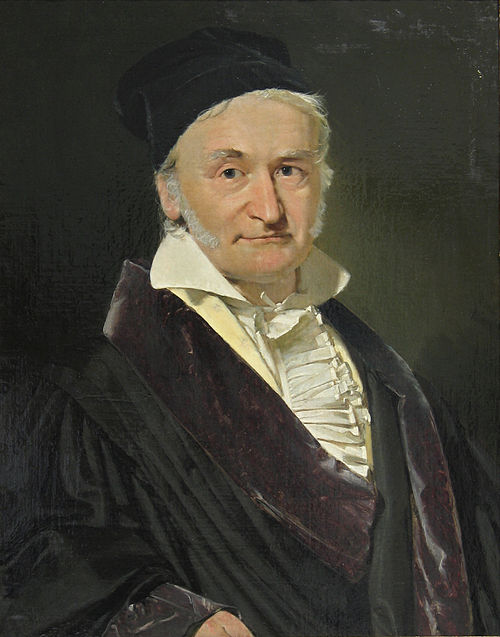
\includegraphics[width=0.65\linewidth]{figures/500px-Carl_Friedrich_Gauss_1840_by_Jensen.jpg}
        \end{figure}
        \end{columns}
        
\end{frame}

\begin{frame}
	\frametitle{Computer-Aided Mathematical Research}

        \begin{columns}
        \column{0.7\textwidth}
            \begin{itemize}
            \item \textbf{Scientific Computation}: Widely used to solve differential equations, dynamical systems and statistics of large matrices
                \begin{itemize}
                    \item Hendrik Lorentz assembled a team of human computers to model the fluid flow around the Afsluitdijk;
                    \item Numerical analysis of Navier–Stokes equations
                \end{itemize}
        \end{itemize}

        \column{0.3\textwidth}
        \begin{figure}
            \centering
            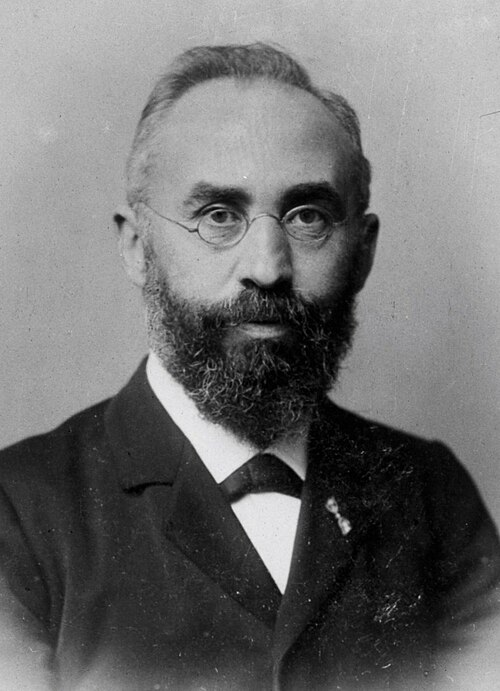
\includegraphics[width=0.65\linewidth]{figures/Nobelprijswinnaars._H.A._Lorentz_(cropped).jpg}
        \end{figure}
        \end{columns}
        
        
\end{frame}

\begin{frame}
	\frametitle{Computer-Aided Mathematical Theorem Proving}
        
        \begin{block}{Four color theorem}
        % \begin{columns}
            % \column{0.6\textwidth}
            Given any separation of a plane into contiguous regions, the regions can be colored using at most four colors so that no two adjacent regions have the same color. (intuitive statement)
            % \column{0.3\textwidth}
        %     \begin{figure}
        %     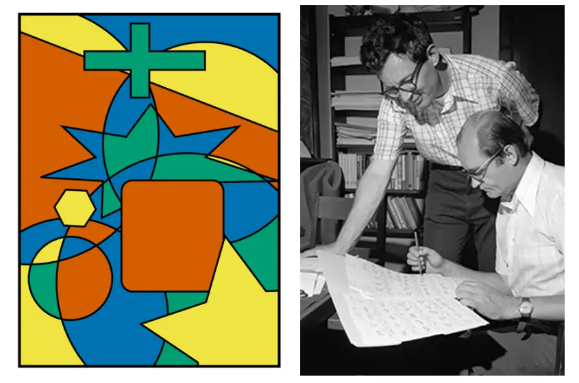
\includegraphics[width=\linewidth]{figures/Four_clours.png}
        % \end{figure}
        % \end{columns}            
        \end{block}
        
        \begin{columns}
        
        \column{0.6\textwidth}
            
        \begin{itemize}
            \item The first major theorem mainly proved with the help of a computer. % \footnote{\small Appel and Haken, "Every Planar Map Is Four Colorable", 1976} 
            \item Computers check the “reducibility” and “unavoidability.” of almost 2000 configurations.
        \end{itemize}

            \column{0.4\textwidth}
            \begin{figure}
                \centering
                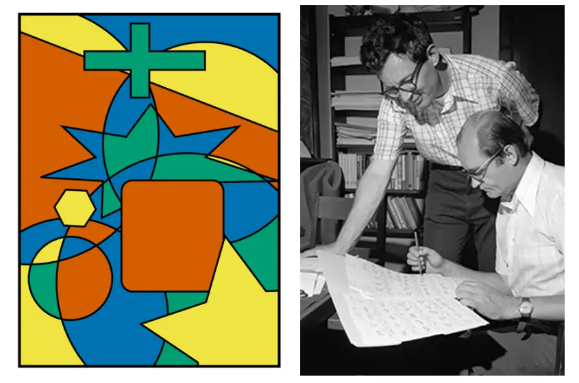
\includegraphics[width=0.9\linewidth]{figures/Four_clours.png}
            \end{figure}
        \end{columns}
        
        
\end{frame}

\begin{frame}
	\frametitle{Computer-Aided Mathematical Theorem Proving}
        \begin{block}{Boolean Pythagorean triples theorem}
            The set $\{1, ..., 7824\}$ can be partitioned into two classes, neither of which contains a Pythagorean triple $(a, b, c)$ with $a^2 + b^2 = c^2$; however, this is not possible for $\{1, ..., 7825\}$.
        \end{block}
        
        \begin{columns}
        
        \column{0.6\textwidth}
        
        \begin{itemize}
            \item The proof required four CPU-years of computation and generated a 200 terabyte propositional proof, which was later compressed to 68 gigabytes. % \footnote{\small Heule, Marijn J. H.; Kullmann, Oliver; Marek, Victor W., "Solving and Verifying the Boolean Pythagorean Triples problem via Cube-and-Conquer", 2016}
            \item It is a typical example of a result proved using a satisfiability (SAT) solvers.
        \end{itemize}

        \column{0.4\textwidth}
            \begin{figure}
                \centering
                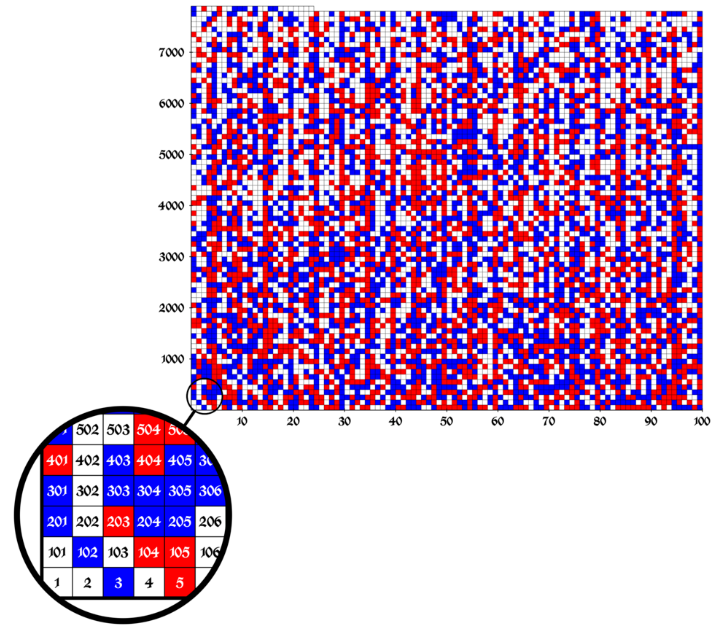
\includegraphics[width=0.7\linewidth]{figures/Triples.png}
            \end{figure}
        \end{columns}

        
\end{frame}

\begin{frame}
\frametitle{Formalized Math in Early Era}
        \begin{columns}
        
        \column{0.6\textwidth}
        
        \begin{itemize}
            \item Leibniz's "universal characteristic" that could be applied across all fields of reasoning;
            \item Hilbert's style of axiomatic approach (although is shown wrong);
            \item Bourbaki's formalized mathematics that highlight the necessary of formalization;
            \item McCarthy's idea that proof checking can be easier and briefer by computer.
        \end{itemize}

        \column{0.4\textwidth}
            \begin{figure}
                \centering
                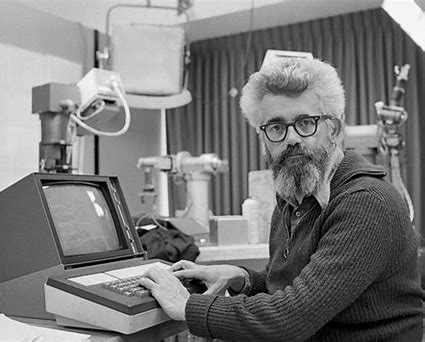
\includegraphics[width=0.8\linewidth]{figures/John_McCarthy.jpg}
            \end{figure}
        \end{columns}
	
\end{frame}

\begin{frame}
	\frametitle{Formalization}

            \begin{columns}
        
        \column{0.7\textwidth}
        
        	\begin{itemize}
		\item \textbf{Necessary of Formalization (Challenges in Math)}: 
                \begin{itemize}
                    \item Complexity:
                        \begin{itemize}
                            \item Lengthy proofs spanning thousands of pages;
                            \item Interdisciplinary problems requiring diverse expertise.
                        \end{itemize}
                    \item Verification:
                        \begin{itemize}
                            \item Time-intensive peer reviews by limited experts;
                            \item High risk of subtle errors being missed.
                        \end{itemize}
                    \item Knowledge Management:
                        \begin{itemize}
                            \item Rapidly growing mathematical literature;
                            \item No single expert can keep up with all advancements.
                        \end{itemize}
                \end{itemize}
            \end{itemize}
            
        \column{0.3\textwidth}
            \begin{figure}
                \centering
                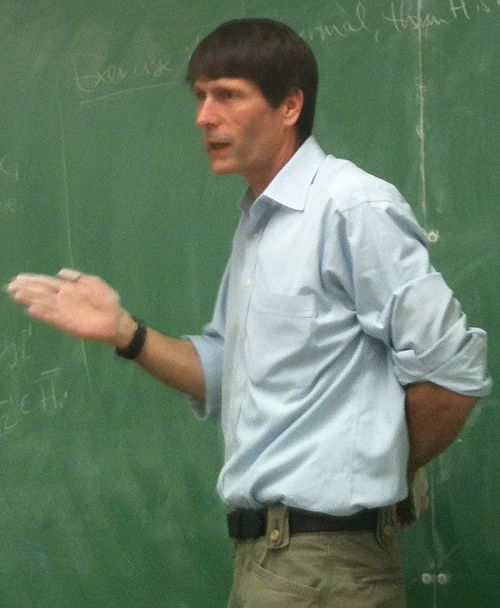
\includegraphics[width=0.68\linewidth]{figures/500px-Halescropped.jpg}
            \end{figure}
        \end{columns}

        \begin{itemize}
            \item An example is that the proof of Kepler conjecture given by Hales is 300 pages long so that a 12-person team spent four years without being able to make a solid judgment on its correctness.
        \end{itemize}
	
\end{frame}

\begin{frame}
	\frametitle{Formalization}

        \begin{columns}
        
        \column{0.7\textwidth}
        
        \begin{itemize}

            \item \textbf{Values of Formalization}: 
            \begin{itemize}
                    \item Provides an extremely high level of confidence that a given result is correct;
                    \item Uncovers minor issues in the human proof, and sometimes reveals simplifications or strengthenings of the argument;
                    \item Contributes many basic mathematical results to a mathematical library during the process;
                    \item Offers a chance that more researchers can be allowed to participate in a project without considering the accuracy of their work.
                \end{itemize}
            
	\end{itemize}

        \column{0.3\textwidth}
            \begin{figure}
                \centering
                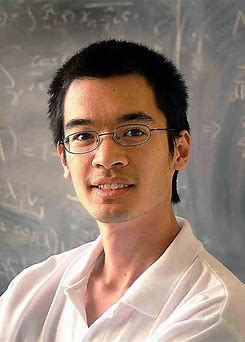
\includegraphics[width=0.72\linewidth]{figures/Tao.jpg}
            \end{figure}
        \end{columns}
    
\end{frame}

\begin{frame}
	\frametitle{Two types of Automated Reasoning and Formal Proofs}
    
            \begin{itemize}
            \item \textbf{Automated theorem proving}: 
                \begin{itemize}
                    \item SMT solvers, model checkers, ATP systems in first-order logic, etc.
                    \item Minimal efforts from humans;
                    \item Limited expressiveness and difficult to scale.
                \end{itemize}
            \end{itemize}
            
        \begin{figure}
            \centering
            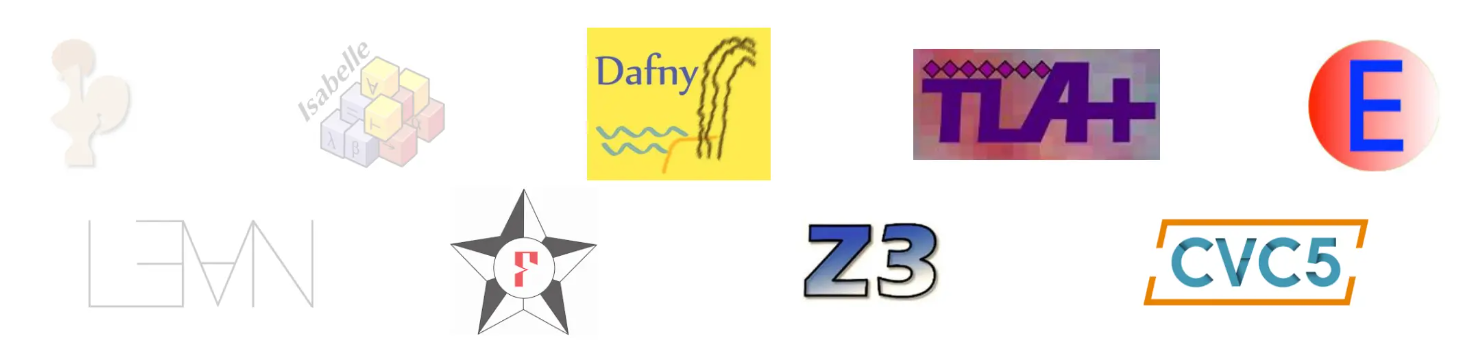
\includegraphics[width=0.8\linewidth]{figures/AutoMath_2.png}
        \end{figure}
        
\end{frame}

\begin{frame}
	\frametitle{Two types of Automated Reasoning and Formal Proofs}
    
            \begin{itemize}
            \item \textbf{Interactive theorem proving}: 
                \begin{itemize}
                        \item Proof assistants such as Coq, Isabelle, and Lean.
                        \item Expressive logic % \footnote{\small Leroy, "Formal Verification of a Realistic Compiler", 2008.}, e.g., dependent type theory and is successfully used in large formalization projects; % \footnote{\small Hales et al., "A Formal Proof of the Kepler Conjecture", 2017.}
                    
                        \item Needs lots of efforts from humans to write formalized proof.
                \end{itemize}
            \end{itemize}

        \begin{figure}
            \centering
            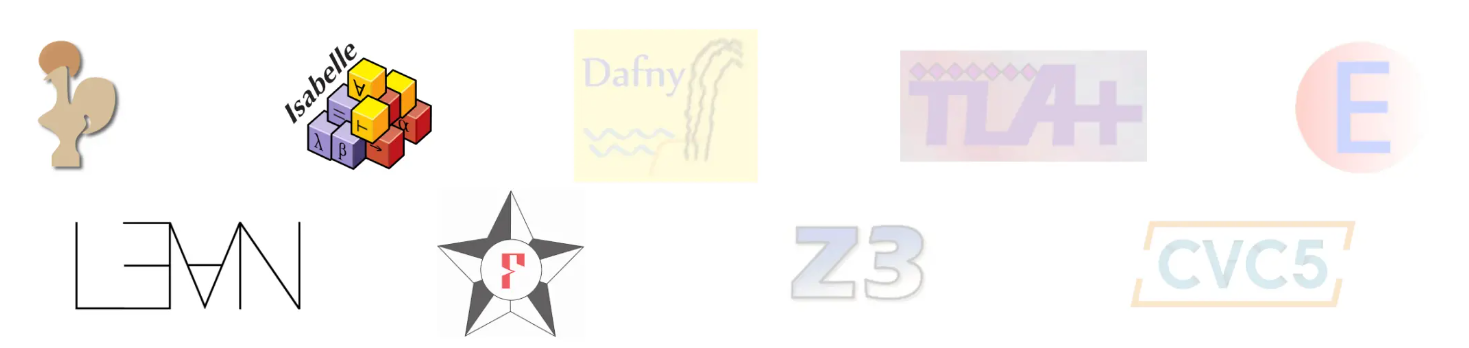
\includegraphics[width=0.8\linewidth]{figures/AutoMath_1.png}
        \end{figure}
        
\end{frame}

\begin{frame}
	\frametitle{An Example of Theorem Proof with Proof Assistants}
            \begin{columns}
                    \column{0.58\textwidth}
            \begin{itemize}
                \item \textbf{natural statement: } 
                    
                    \(\forall n \in \mathbb{N}\), the greatest common divisor of \(n\) and itself is \(n\) itself.
                \item \textbf{Lean statement: } 
                    
                    Theorem gcd\_self (n : nat) : gcd n n = n :=
                    
                    begin
                    
                    \qquad cases n,
                    
                    \qquad \{ unfold gcd \},
                    
                    \qquad unfold gcd,
                    
                    \qquad rewrite mod\_self,
                    
                    \qquad apply gcd\_zero\_left
                    
                    end

                   
                    
            \end{itemize}

             \column{0.4\textwidth}
                    \begin{figure}
                        \centering
                        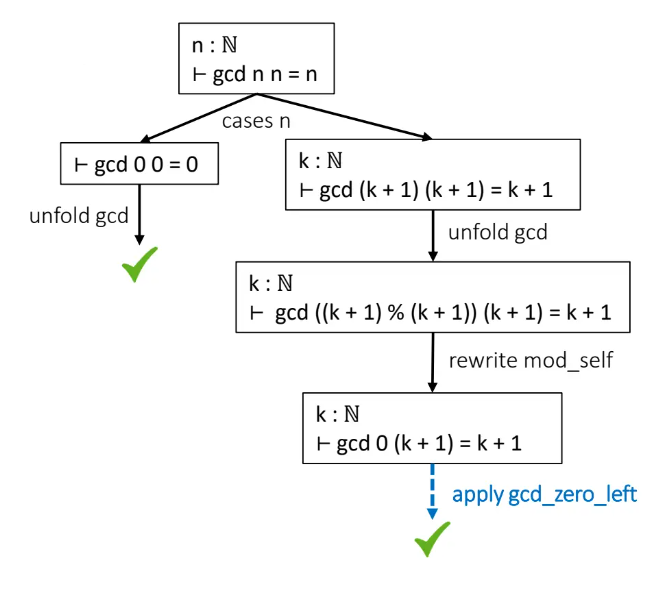
\includegraphics[width=0.9\linewidth]{figures/AP.png}
                    \end{figure}
            \end{columns}
            
                    
    
\end{frame}

\begin{frame}
	\frametitle{Capabilities of LLMs on Science}

        \begin{itemize}
            \item The capabilities of LLMs in solving these problems have significantly improved from 2023 to 2025 on the GPQA Diamond, a benchmark for measuring PhD-level scientific questions.
        \end{itemize}
        \begin{figure}
            \centering
            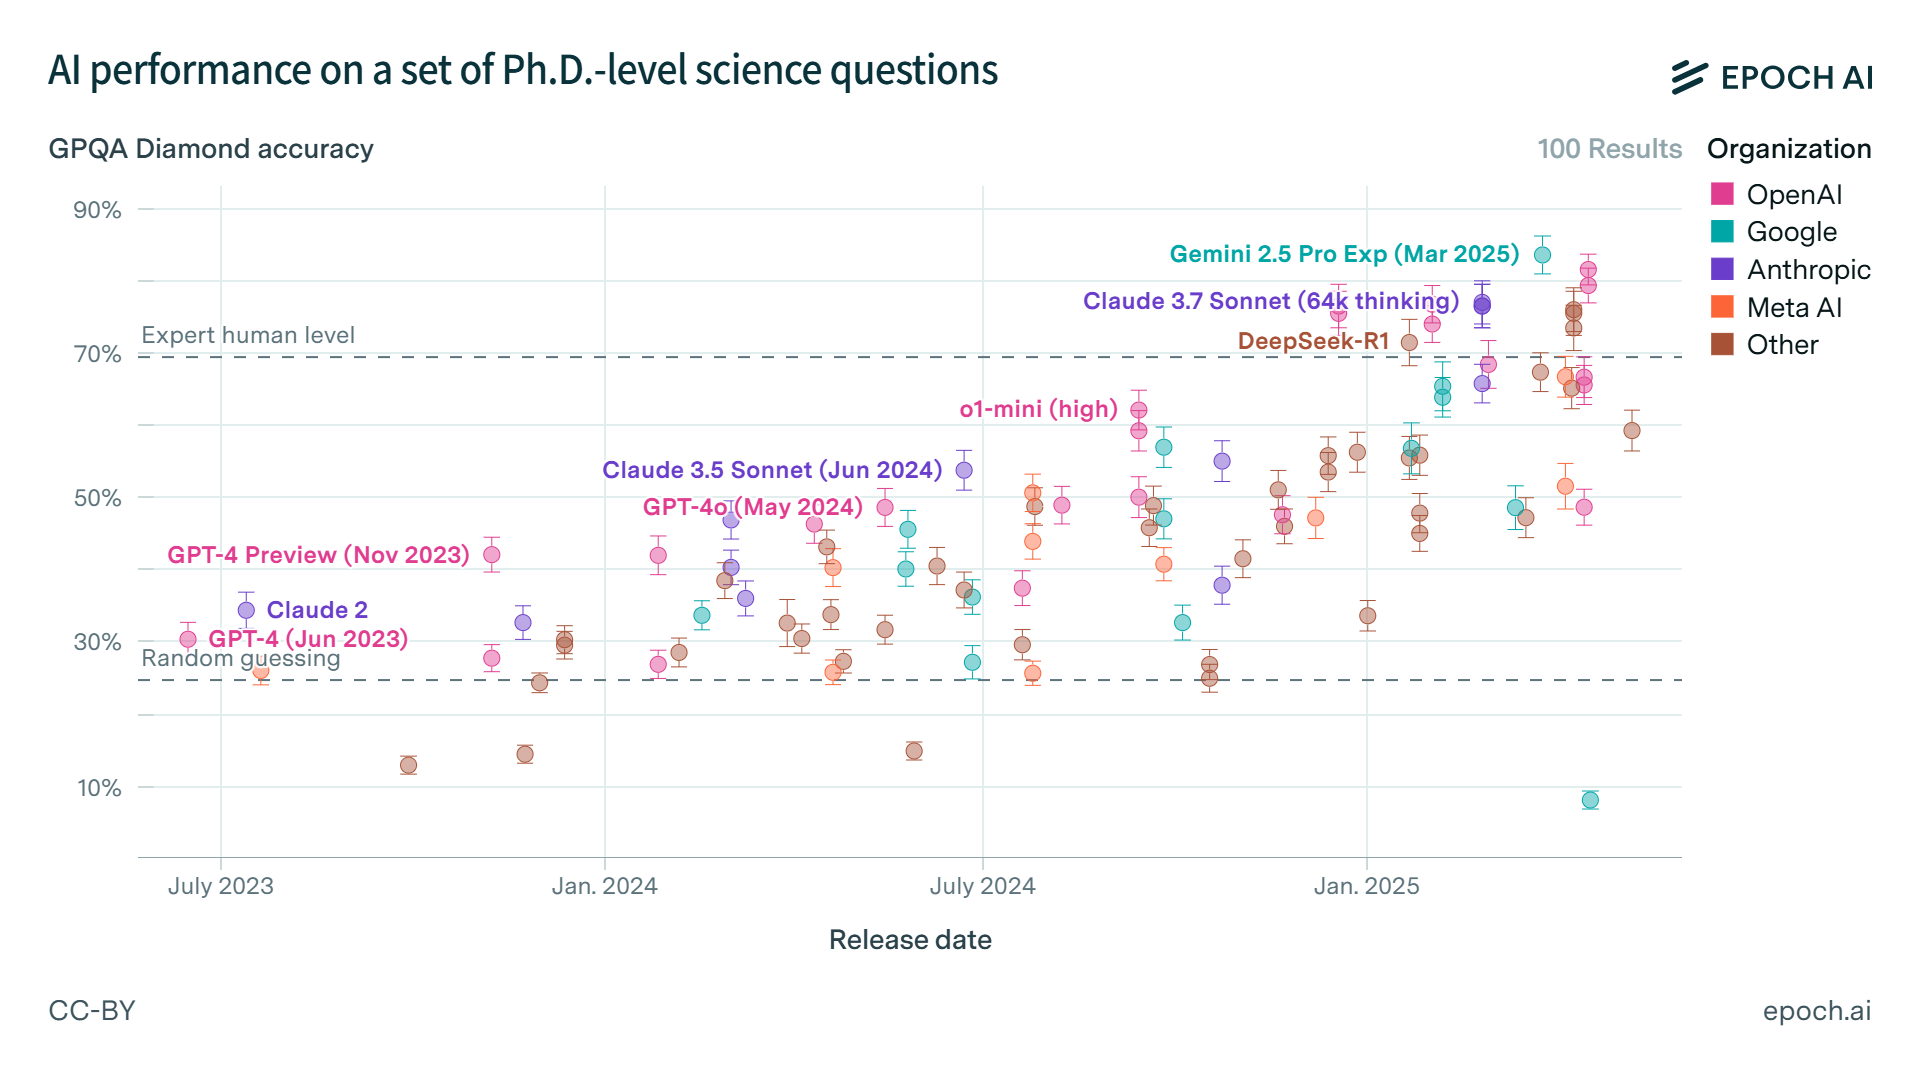
\includegraphics[width=0.6\linewidth]{figures/benchmarks.png}
        \end{figure}
        
\end{frame}


\begin{frame}
	\frametitle{Capabilities of LLMs on Math}

        \begin{itemize}
            \item DeepMind's AlphaProof, a model for formal theorem proving, along with AlphaGeometry 2, a model focused on geometry, scored 28 and 25 points respectively in IMO 2024, just 1 point short of gold - medal level.
                
        \end{itemize}
        \begin{figure}[H]
        \centering
        \begin{minipage}[b]{0.75\linewidth}
            \subfigure[Performance of AlphaProof]{
                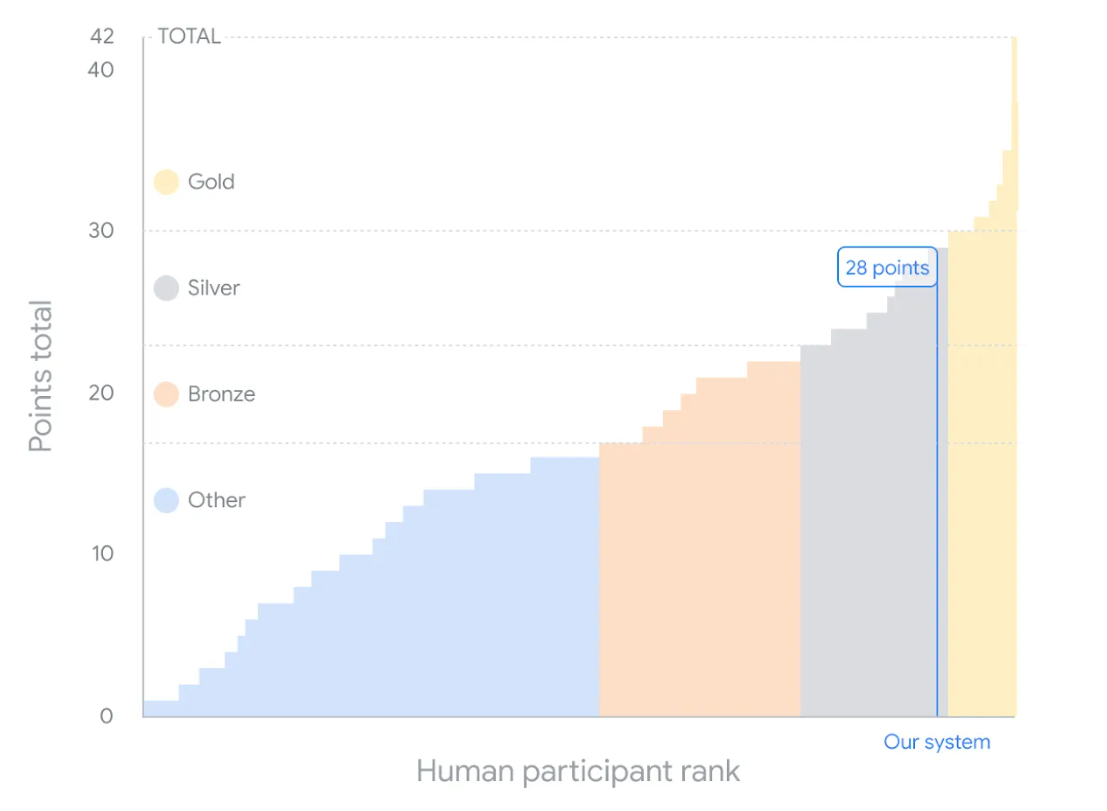
\includegraphics[width=0.42\linewidth]{figures/Scores of AP.png}
            }
            \subfigure[Performance of AlphaGeometry]{
                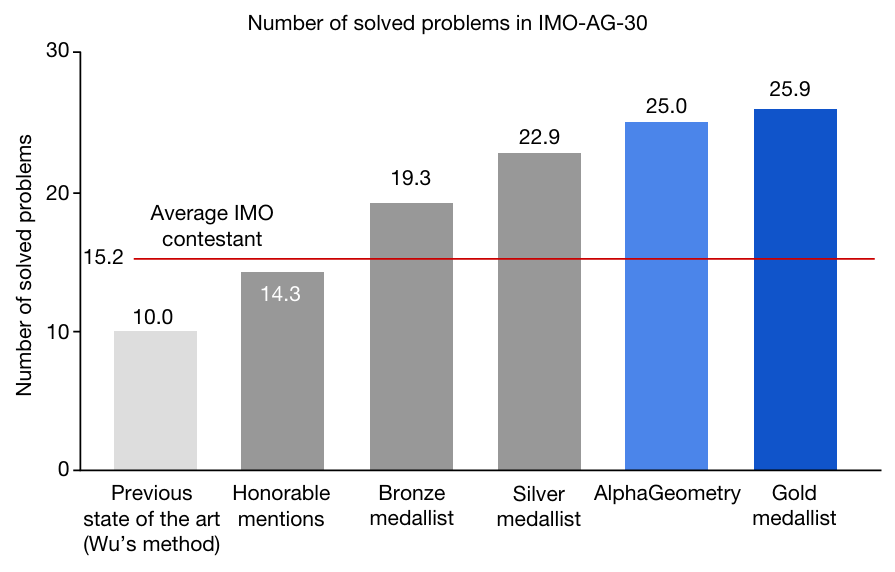
\includegraphics[width=0.52\linewidth]{figures/Scores of AG1.png}
      }
        \end{minipage}
  \end{figure}
  
\end{frame}



\begin{frame}
	\frametitle{How to Generate Reliable Results with LLMs on Math}
        \begin{columns}
            \column{0.4\textwidth}
             \begin{itemize}
                    \item Generate a step of proof including static and possible premises rather than to try building the whole proof directly;% \footnote{\small Kaiyu Yang et al.,“LeanDojo: Theorem Proving with Retrieval-Augmented Language Models”,2023.}
                    \item Enhance existing symbolic proof engines to attack narrow classes of mathematics problems.% \footnote{\small Trieu H. Trinh et al.,“Solving olympiad geometry without human demonstrations”,2024.} 
                \end{itemize}
            \column{0.6\textwidth}    
            \begin{figure}
            \centering
            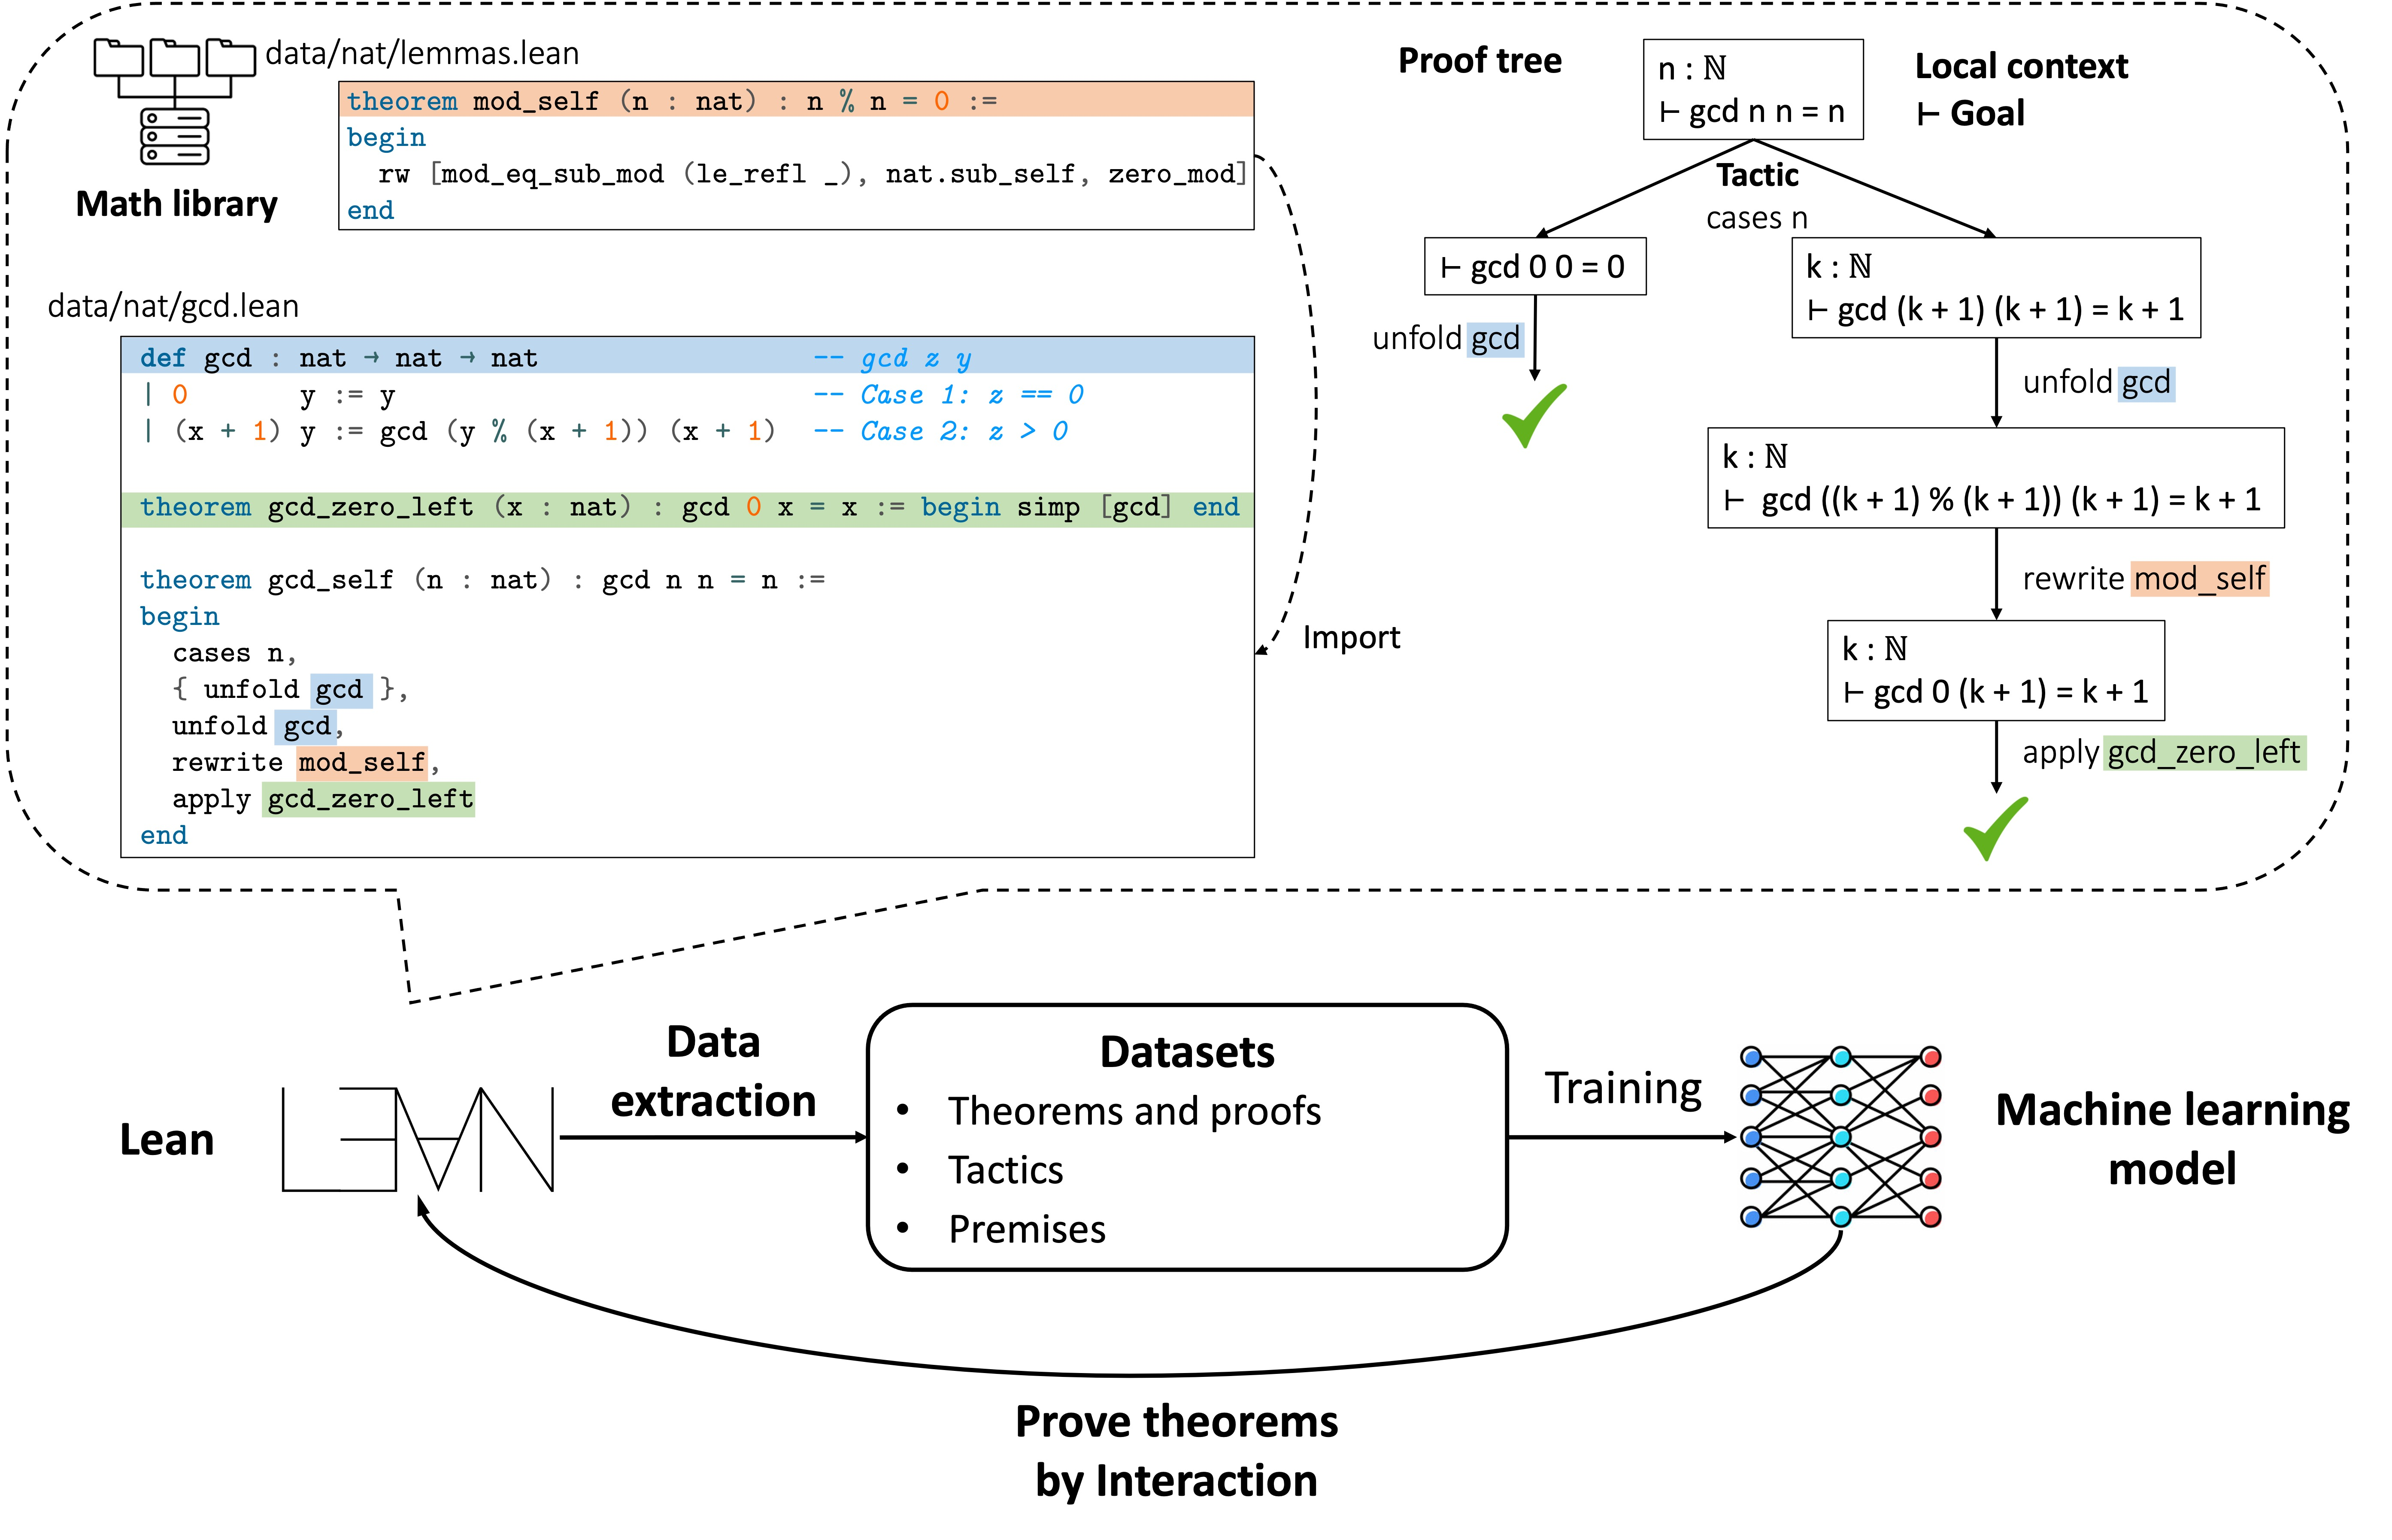
\includegraphics[width=0.9\linewidth]{figures/LeanDojo.jpg}
        \end{figure}
        \end{columns}
               


\end{frame}

\begin{frame}
	\frametitle{Reasons for Choosing Euclidean Plane Geometry}

        \begin{itemize}
            \item Clear and axiomatized system allows for the formalization and systematization of geometric theorem proofs, making them easier for computer to perform symbolic reasoning and verify;
            \item The proof often requires creative construction of auxiliary points, which can be given by LLMs;
            \item It would be possible to attempt to have LLMs derive most of the theorems in Euclidean plane geometry symbolically from the most basic axioms and compare them with the content constructed by humans.
        \end{itemize}
        
  
\end{frame}


\section{Related Work}
\begin{frame}
	\frametitle{Wu's Method}
        \begin{columns}
            \column{0.7\textwidth}
            \begin{itemize}
	    \item \textbf{Introduction}:
        
        Wu's Method is a symbolic computation method for the automatic proof of geometric theorems based on algebraic geometry and polynomial elimination theory, primarily utilizing pseudodivision to transform conditional polynomials into a triangular form, and then using symbolic computation and logical reasoning to prove geometric theorems.
	\end{itemize}
            \column{0.3\textwidth}
            \begin{figure}
                \centering
                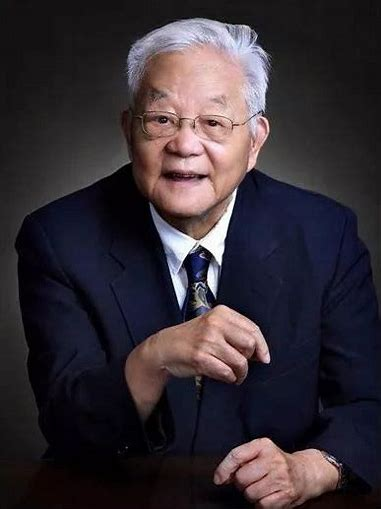
\includegraphics[width=0.65\linewidth]{figures/Wu.jpg}
            \end{figure}
        \end{columns}
	
    
\end{frame}

\begin{frame}
	\frametitle{Wu's Method}
	\begin{itemize}
	    
            \item \textbf{The form of the Transcribed Problem}: \[\forall x, y, z, \ldots I(x, y, z, \ldots) \implies f(x, y, z, \ldots)\]
            where \(f\) is a polynomial equation and \(I\) is a conjunction of polynomial equations. The algorithm is complete for such problems over the complex domain.
            
            \item \textbf{Brief Introduction of Algorithm}: For an ideal \(I\) in the ring \(K[x_1, x_2, \dots, x_n]\) over a field \(K\), a (Ritt) characteristic set \(C\) of \(I\) is composed of a set of polynomials in I, which is in triangular shape. Given a characteristic set \(C\) of \(I\), one can decide if a polynomial \(f\) is zero modulo \(I\).
            
	\end{itemize}
    
\end{frame}

\begin{frame}
	\frametitle{An Easy Example with Wu's Method}
        \begin{itemize}
            \item \textbf{Problem} 

            As shown in figure, let circles $O_1$ and $O_2$ intersect at points $A$ and $B$. Take any point $C$ on the line containing $A$ and $B$. Draw tangents $CT_1$ and $CT_2$ from $C$ to circles $O_1$ and $O_2$ respectively. Show that \(|CT_1| = |CT_2|\).
        
            \begin{figure}
            \centering
            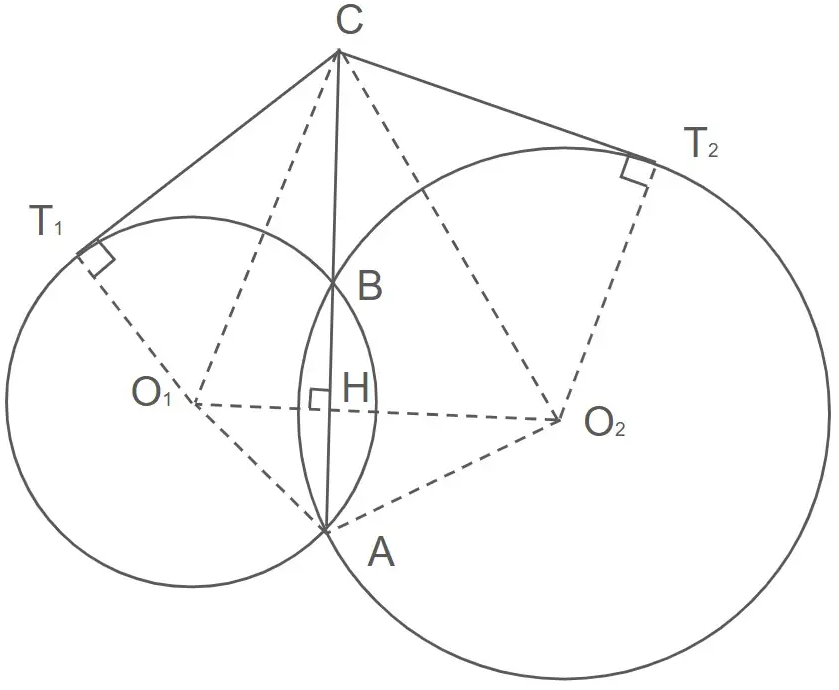
\includegraphics[width=0.3\linewidth]{figures/Wu.png}
        \end{figure}

        \end{itemize}
    
\end{frame}

\begin{frame}
	\frametitle{An Easy Example with Wu's Method}
        \begin{itemize}
        \item \textbf{Natural Proof} 
        
        The length of the tangent are $CT_1^2 = CO_1^2 - O_1T_1^2 = CO_1^2 - O_1A^2$ and $CT_2^2 = CO_2^2 - O_2A^2$.
        
        Connect $O_1O_2$ and let it intersect $AB$ at point $H$. Since $A$ and $B$ are the intersection points of the two circles, $O_1O_2 \perp AB$.
        
        Thus we have $CO_1^2 - O_1A^2 = CO_2^2 - O_2A^2$, which implies $CT_1 = CT_2$.
        
        \end{itemize}
    
\end{frame}

\begin{frame}
	\frametitle{An Easy Example with Wu's Method}
        \begin{itemize}
            \item \textbf{Wu's Method Proof} 

            Assume the plane is the complex plane, the coordinates of $O_1$, $O_2$ are $z_1$, $z_2$ and the radii are $r_1$,  $r_2$. Then solve for the coordinates of $A,B$ and the equation of that line by combining the equations of the circles:
        \begin{align*}
        O_1: \quad & (z - z_1)(\bar{z} - \bar{z}_1) = r_1^2 \\
        O_2: \quad & (z - z_2)(\bar{z} - \bar{z}_2) = r_2^2
        \end{align*}

        The result of subtracting the two equations is the equation of the line $AB : z(\bar{z}_2 - \bar{z}_1) + \bar{z}(z_2 - z_1) + (z_1\bar{z}_1 - z_2\bar{z}_2) = r_1^2 - r_2^2$.

        The equality of the lengths of the tangents is equivalent to verifying the polynomial:
        \begin{align*}
        f(z) = (|z - z_1|^2 - r_1^2) - (|z - z_2|^2 - r_2^2)
        \end{align*}
        is equal to 0 when $z \in AB$.
        
        \end{itemize}
    
\end{frame}

\begin{frame}
	\frametitle{Wu's Method}
	\begin{itemize}
	    \item \textbf{Characteristics}:
                \begin{itemize}
                    \item The proof process of Wu's method is clearly algorithmic and can be easily implemented on a computer, e.g. mathematica;
                    \item Automatically identify the non-degenerate conditions of the problems.
                \end{itemize}
            \item \textbf{Disadvantages}: 
                \begin{itemize}
                    \item For enough complex problem, the scale and degrees of polynomials are large and high , which consume a large amount of computational resources and time;
                    \item Its highly mechanized process makes it difficult for human to read and understand;
                    \item When condition comes to inequality, it struggles to handle them effectively.
                \end{itemize}
	\end{itemize}
\end{frame}

\section{AlphaGeometry}
\begin{frame}
	\frametitle{AlphaGeometry}
	\begin{itemize}
	    \item An AI system developed by Google DeepMind to solve complex geometry problems.
            \item In a benchmark test of 30 Olympiad-level geometry problems, AlphaGeometry1 solved 25, compared to the human gold - medalists' average of 25.9. % \footnote{\small Trieu H. Trinh et al.,“Solving olympiad geometry without human demonstrations”,2024.}. Now AlphaGeometry2 solved 42 on a benchmark test of 50 Olympiad-level geometry problems. % \footnote{Yuri Chervonyi et al., "Gold-medalist Performance in Solving Olympiad Geometry with AlphaGeometry2",2025}
	\end{itemize}

    \begin{figure}
        \centering
        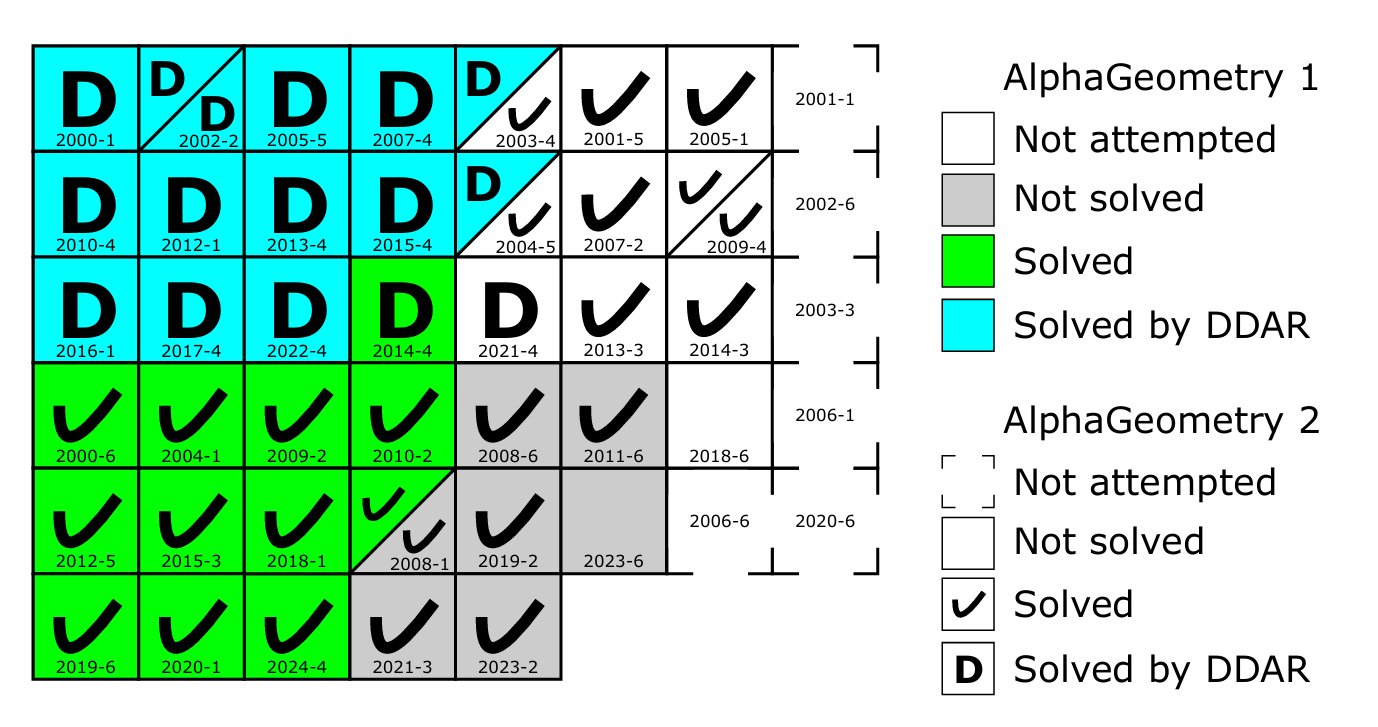
\includegraphics[width=0.5\linewidth]{figures/AlphaGeo.png}
    \end{figure}
\end{frame}

\begin{frame}
	\frametitle{AlphaGeometry}
	\begin{itemize}
	    \item AlphaGeometry's geometric problem-solving process consists of formalization, Symbolic Deduce and Auxiliary Construction offered by LM, covering simple problems and the 2015 IMO P3 solution.
	\end{itemize}

    \begin{figure}
        \centering
        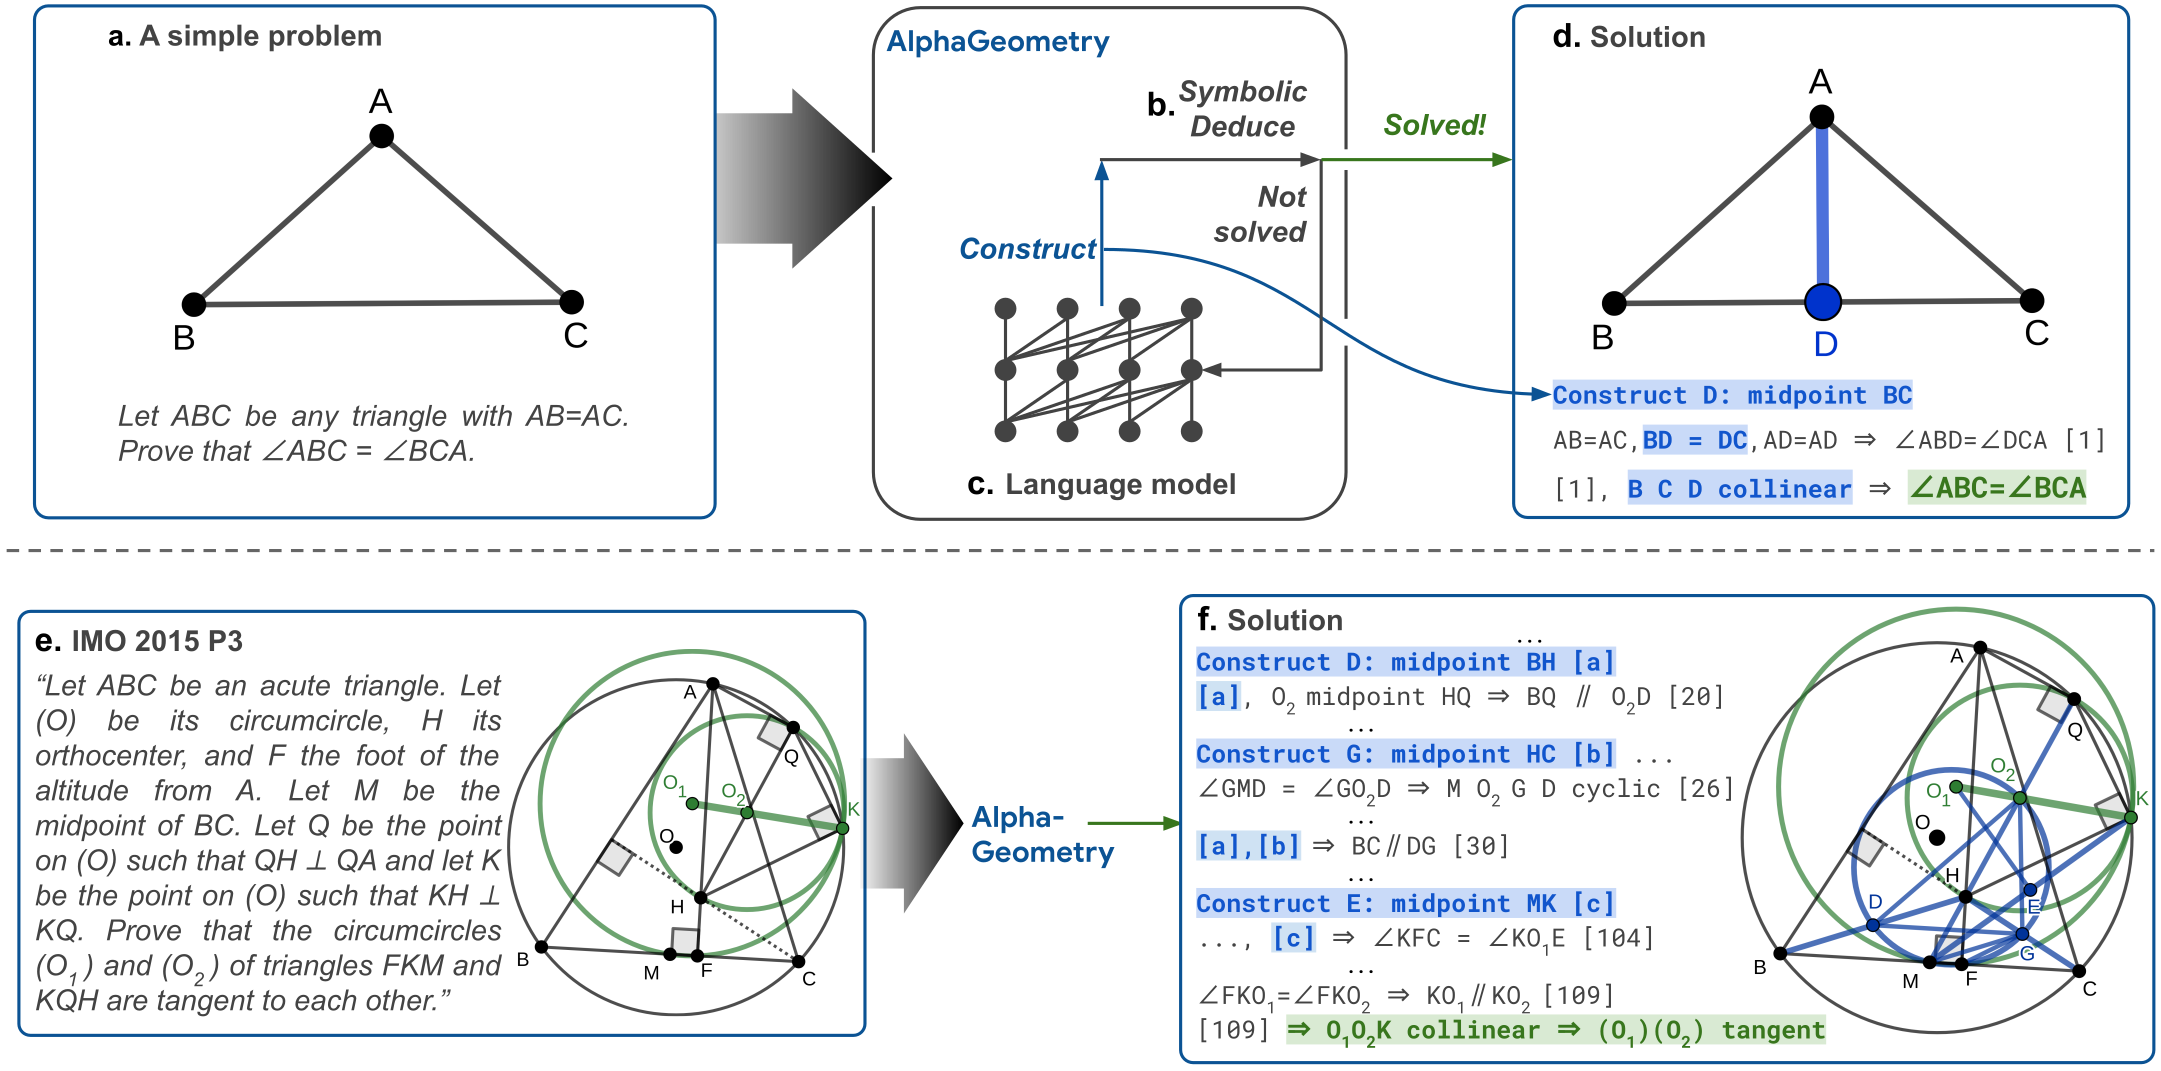
\includegraphics[width=0.7\linewidth]{figures/AG1.png}
    \end{figure}
\end{frame}

\begin{frame}
	\frametitle{AlphaGeometry}
        \textbf{Detailed Process description of problems solving in AG}
	\begin{enumerate}
	    \item Input a formalized geometry problem;
            \item Do \textbf{Deductive Database} (DD) and \textbf{Algebraic Reasoning} (AR) to gain a deduction closure and new algebraic relationships respectively;

            \item If the target conclusion is in the deduction closure, the problem is proven.
            \item If not, feed the new algebraic relationships given by AR back to DD to further expand the deduction closure (step 3).
            \item If the target conclusion is still not in the new deduction closure, then use LM to generate auxiliary constructions (points) and back to step 2.
	\end{enumerate}

\end{frame}

\begin{frame}
        \frametitle{Domain Special Language (DSL)}
        In AlphaGeometry (AG), Below are the main components and features of the formalization language:
	\begin{itemize}
            \item \textbf{Basic Elements}
                \begin{itemize}
                    \item \textbf{Points}: Represented by single lowercase letters, e.g., \texttt{a}.
                    \item \textbf{Lines}: Represented by two points, e.g., \texttt{line a b} denotes the line passing through points \texttt{a} and \texttt{b}.
                    \item \textbf{Circles}: Represented by a center and a point on the circumference, e.g., \texttt{circle a b} denotes a circle centered at point \texttt{a} and passing through point \texttt{b}.
                \end{itemize}
        \end{itemize}
\end{frame}

\begin{frame}
        \frametitle{Domain Special Language (DSL)}
	\begin{itemize}
            \item \textbf{Relations and Predicates}
                
                The AG language uses a set of relations and predicates to describe the properties and interactions between geometric objects.
                \begin{itemize}
                \item \textbf{Collinearity}: \texttt{coll a b c} indicates that points \texttt{a}, \texttt{b}, and \texttt{c} are collinear.
                \item \textbf{Concyclicity}: \texttt{cyclic a b c d} indicates that points \texttt{a}, \texttt{b}, \texttt{c}, and \texttt{d} are concyclic.
                \item \textbf{Equality of Distances}: \texttt{cong a b c d} indicates that line segment \texttt{ab} is equal to line segment \texttt{cd}.
                \item ...
                \end{itemize}
        \end{itemize}
        \begin{figure}
            \centering
            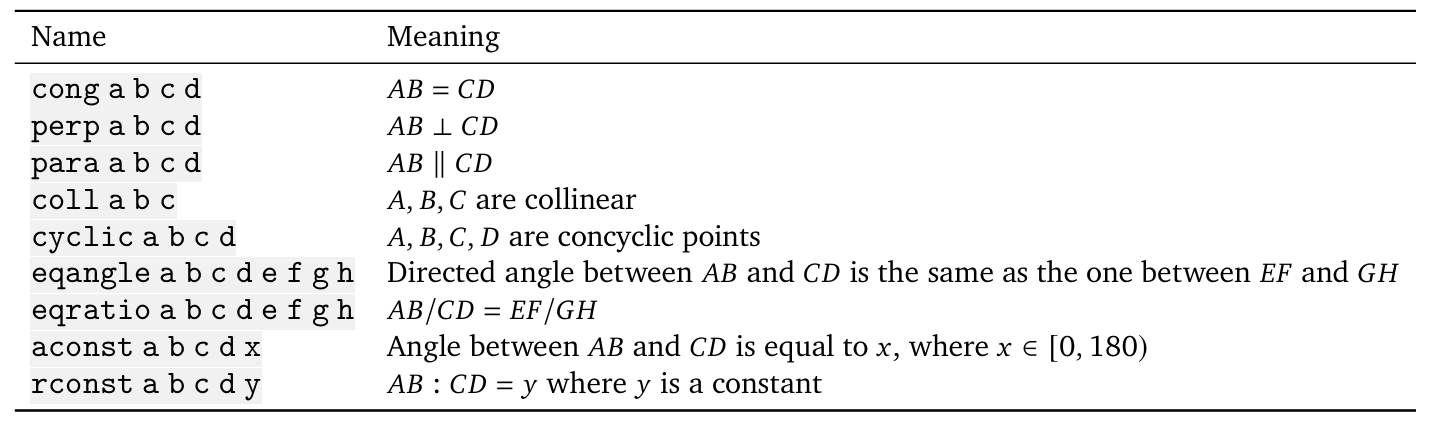
\includegraphics[width=0.65\linewidth]{figures/some_predicates.png}
        \end{figure}
\end{frame}

\begin{frame}
        \frametitle{Symbolic Deduce}
        The Symbolic Deduce is formed by the following two parts:
	\begin{itemize}
            \item \textbf{Deductive Database (DD)}:
            
            A rule-based reasoning system that derives new geometric facts from given premises. It expands the set of known facts by applying a series of predefined geometric rules until the target conclusion is reached or no new facts can be derived. % \footnote{Ye, Z., Chou,"Automated Deduction in Geometry", 2011}

            \item \textbf{Algebraic Reasoning (AR)}:
            
            An algebra-based reasoning engine used to handle algebraic relationships in geometric problems, such as calculations involving angles, ratios, and distances.

        \end{itemize}
\end{frame}

\begin{frame}
        \frametitle{Symbolic Deduce}

            \begin{itemize}
             \item \textbf{Rules in DD}:
                
                derivation rules are as follows: \(predicate + predicate + \ldots \Rightarrow predicate\), where conclusions are drawn from multiple premises. 
                
            \item \textbf{Example}: 
            
            cong O A O B, cong O B O C, cong O C O D \(\Rightarrow\) cyclic A B C D

        \end{itemize}
\end{frame}

\begin{frame}
        \frametitle{Symbolic Deduce}
	\begin{itemize}

            \item \textbf{Details in AR}:
                
                One core of AR is converting the input linear equations to a matrix of their coefficients \(A \in \mathbb{R}^{M \times N}\), where \(N\) and \(M\) are the number of variables and equations respectively.

                In geometry, any equality is of the form  \( a - b = c - d \Leftrightarrow a - b - c + d = 0 \), so AR populate the row for each equality at columns of matrix \(A\), then Gaussian elimination on \( A \) returns a new matrix with leading 1s at each of the columns, essentially representing each variable as a unique linear combination of all remaining variables. 
                
                \item \textbf{Example}:  Consider \( a - b = b - c \), \( d - c = a - d \) and \( b - c = c - e \), then AR can get:
                \[
\begin{pmatrix}
a & b & c & d & e \\
1 & -2 & 1 & 0 & 0 \\
-1 & 0 & -1 & 2 & 0 \\
0 & 1 & -2 & 0 & 1
\end{pmatrix}
\xrightarrow{GE}
\begin{pmatrix}
a & b & c & d & e \\
1 & 0 & 0 & -1.5 & 0.5 \\
0 & 1 & 0 & -1 & 0 \\
0 & 0 & 1 & -0.5 & -0.5
\end{pmatrix}
\Rightarrow
\begin{cases}
a = 1.5d - 0.5e \\
b = d \\
c = 0.5d + 0.5e
\end{cases}
\]
    
    From this result, AR can deterministically and exhaustively deduce all new equalities.
        \end{itemize}
\end{frame}

\begin{frame}
        \frametitle{Symbolic Deduce}

            \begin{itemize}
             \item \textbf{Proof State Graph}:
                
                A graph with geometric objects as nodes and relationships between geometric objects as edges. 
                
                It is used to record all the geometric objects and their relationships that appear during the current deduction process , providing data records for the traceback operations during the execution of DD and AR to generate proofs.
        \end{itemize}
        \begin{figure}
            \centering
            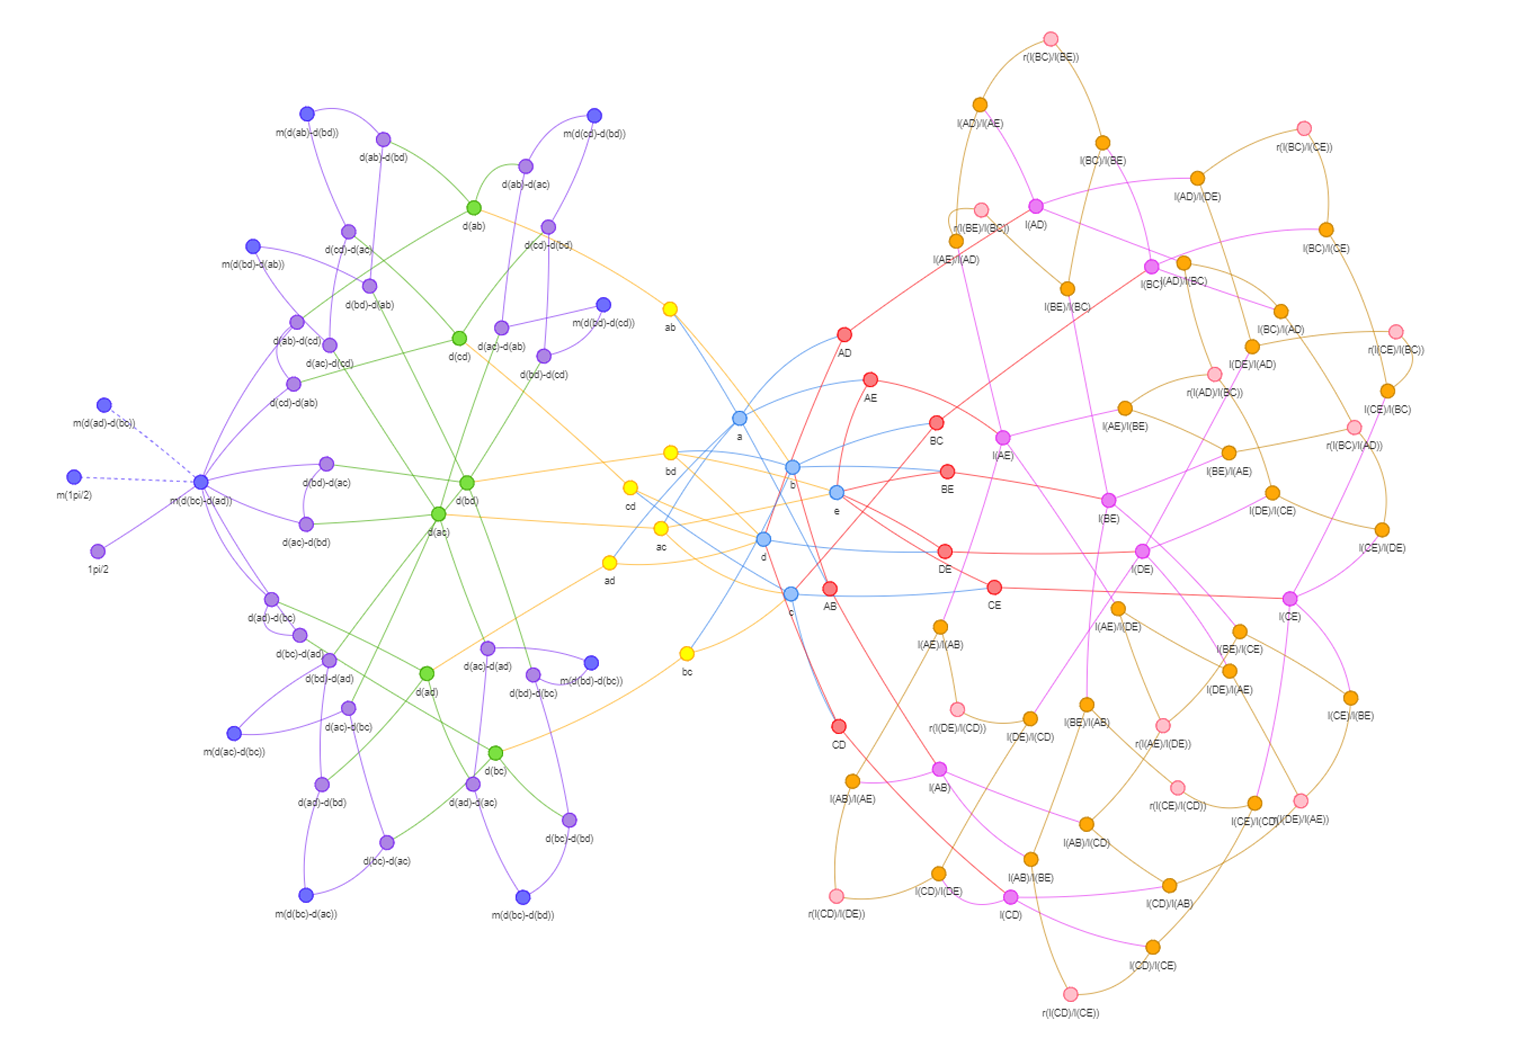
\includegraphics[width=0.45\linewidth]{figures/state graph.png}
        \end{figure}
        
\end{frame}

\begin{frame}
        \frametitle{Symbolic Deduce}

            \begin{itemize}
             \item \textbf{Traceback}:
                
                "Traceback" is a crucial process used for generating proofs for geometric problems. It mainly involves two aspects: DD and AR.

                The goal of traceback is to find the minimal premise conditions required to prove these relationships.

        \end{itemize}
        
        \begin{figure}
            \centering
            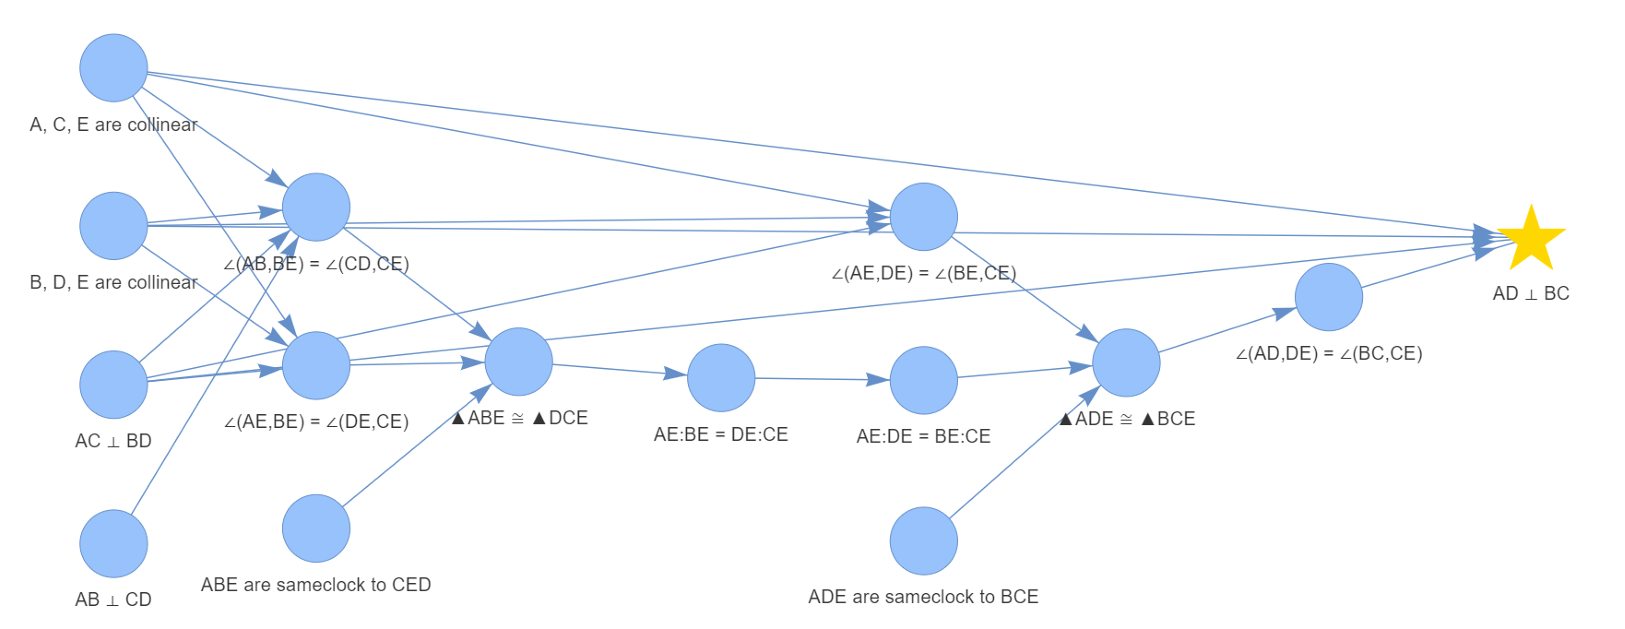
\includegraphics[width=0.6\linewidth]{figures/Graph of state.png}
        \end{figure}
\end{frame}

\begin{frame}
        \frametitle{Symbolic Deduce}

            \begin{itemize}
             \item \textbf{Traceback for DD}:
                \begin{itemize}
                    \item \textbf{Method}: 
                    
                    By recording the equality transitivity graph, the system can track equivalence relationships from one geometric object to another. This process generates a directed acyclic graph (DAG), where each node represents a geometric fact or proposition.

                    \item \textbf{Optimization}: 
                    
                    Finding the shortest path of transitivity is equivalent to finding a minimum spanning tree (MST) for the target set \(S\) of nodes whose weight is the cardinality of the union of its hyperedges \(e'\): 
                    \[
                    \text{MST}(S) = \min_{T \subset E} \left| \bigcup_{e' \in T} w(e') \right| \; \text{ s.t. } \; S \subset T
                    \]
                    This is an NP-hard problem, and AlphaGeometry uses a greedy algorithm to find an approximate minimum spanning tree.
                \end{itemize}

        \end{itemize}
\end{frame}

\begin{frame}
        \frametitle{Symbolic Deduce}

            \begin{itemize}
             \item \textbf{Traceback for AR}:
                \begin{itemize}
                    \item \textbf{Method}: 
                    
                    By recognizing that it is equivalent to a mixed integer linear programming problem, Gaussian elimination can be used to identify equivalences. Given the coefficient matrix of input equations \(A\) and a target equation with coefficients vector \(b \in \mathbb{R}^n\), define non-negative integer decision vectors \(x, y \in \mathbb{Z}^n\) and solve the corresponding mixed-integer linear programming problem:
                    \[
                        x, y = \min_{x,y} \sum_i (x_i + y_i) \ \; \text{ s.t. } \; \ A^T (x - y) = b
                    \]
                    The minimal set of immediate parent nodes for the equivalence represented by \(b\) will be the \(i\)-th equations (ith rows in \(A\)) whose corresponding decision value \((x_i - y_i)\) is non-zero.
    
                \end{itemize}

        \end{itemize}
\end{frame}

\begin{frame}
        \frametitle{Auxiliary Constructions Given by LM}
        \begin{itemize}
            \item In many complex geometric problems, symbolic reasoning engines  alone may not be able to directly prove the target conclusion. So the LM is required to get a formalized problem and then generate one or more descriptions of auxiliary points helping derive the target conclusion.
            \item The number of problems requiring auxiliary points reaches 11 in AG.
        \end{itemize}
        \begin{figure}
            \centering
            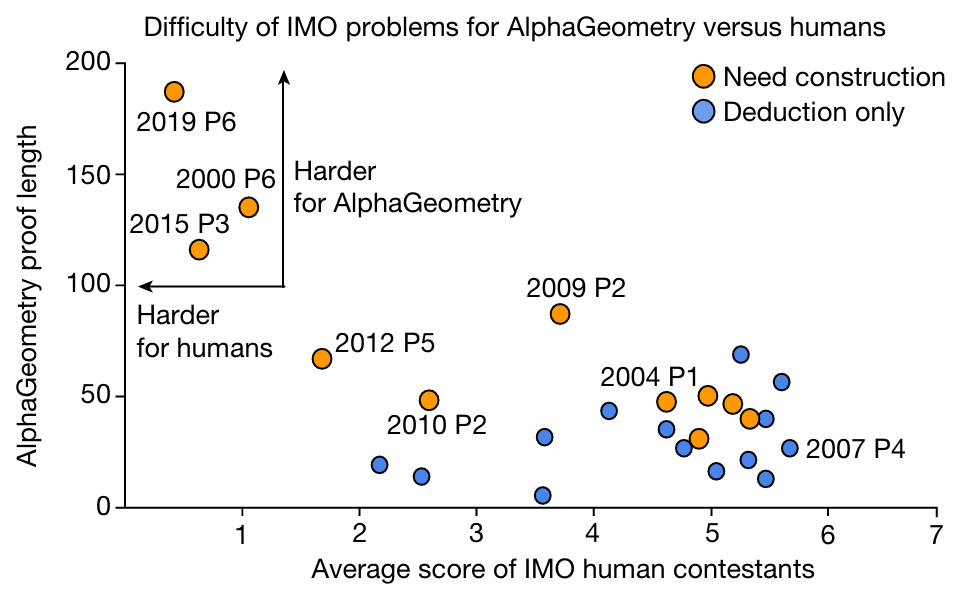
\includegraphics[width=0.5\linewidth]{figures/Proportion of An.png}
        \end{figure}
	
\end{frame}

\begin{frame}
        \frametitle{Synthetic-data-generation in AG}
        \begin{itemize}
            \item AlphaGeometry's synthetic data generation process is formed by three key steps:
                \begin{itemize}
                    \item Sample Random Premises;
                    \item Symbolic Deduction and Traceback;
                    \item Synthetic Problems and Proofs
                \end{itemize}
        \end{itemize}
        \begin{figure}
            \centering
            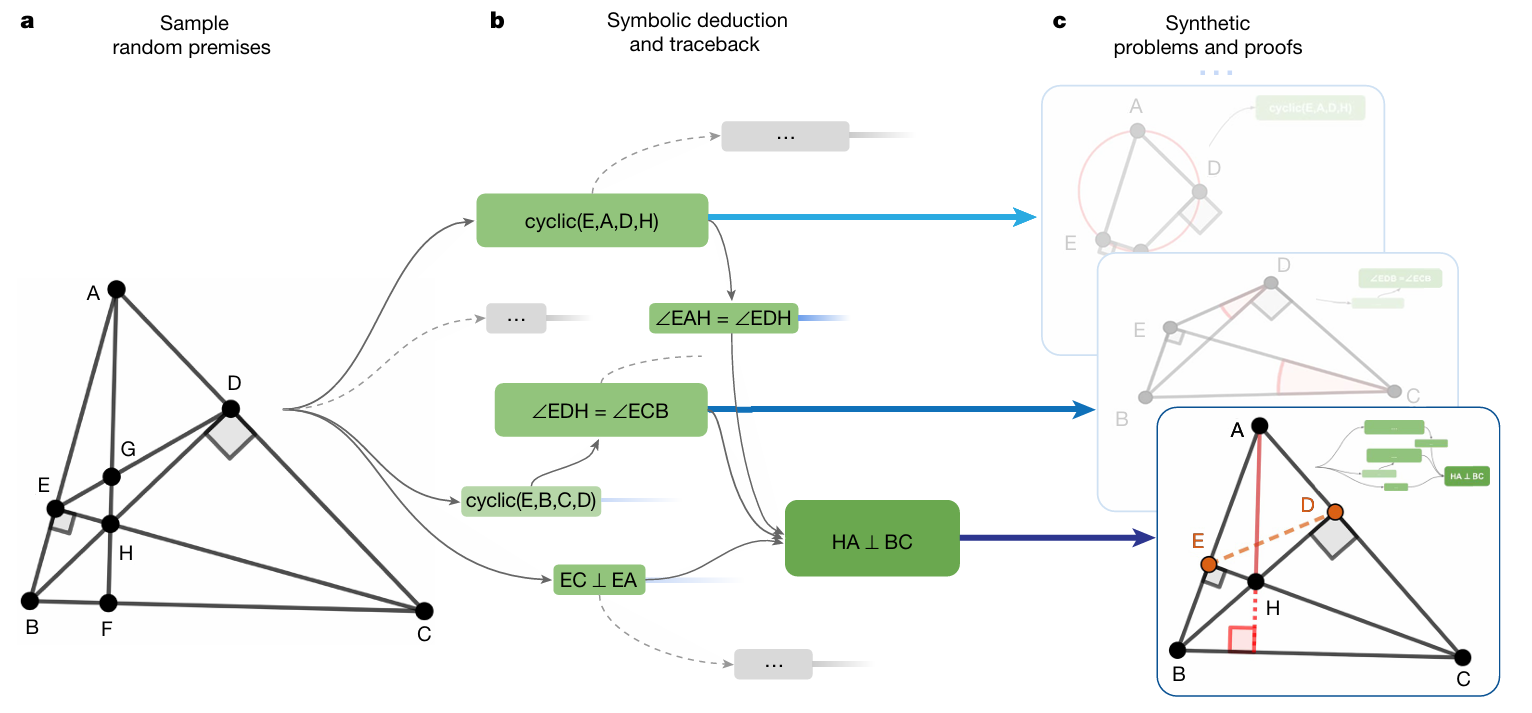
\includegraphics[width=0.65\linewidth]{figures/Data generation.png}
        \end{figure}
	
\end{frame}

\begin{frame}
        \frametitle{Synthetic-data-generation in AG}
        \begin{itemize}
            \item Sample Random Premises:

            The system samples a large set of random theorem premises, which are used as the foundational conditions for generating geometric problems.
        \end{itemize}
        \begin{figure}
            \centering
            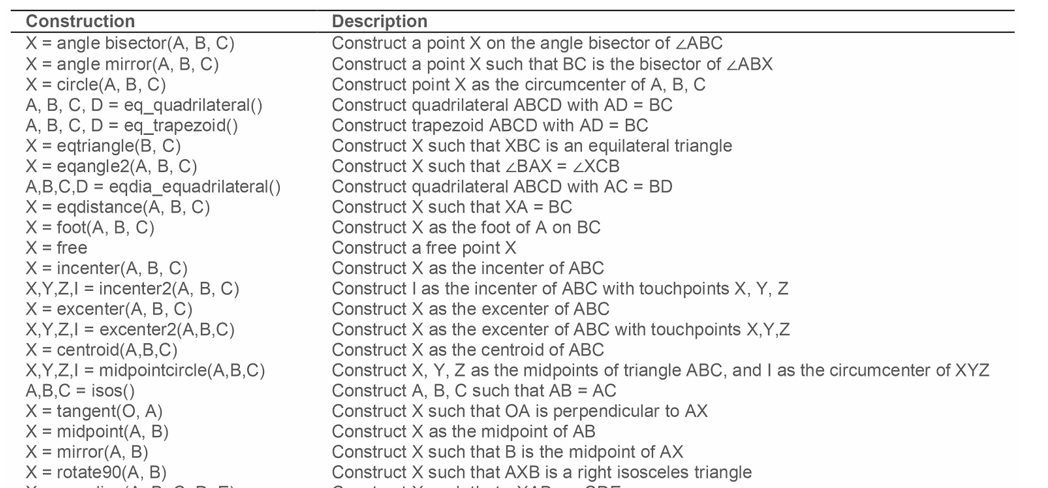
\includegraphics[width=0.6\linewidth]{figures/Actions to construct.png}
        \end{figure}
	
\end{frame}

\begin{frame}
        \frametitle{Synthetic-data-generation in AG}
        \begin{itemize}
            \item Symbolic Deduction and Traceback:

            The symbolic deduction engine (DD and AR) is used to derive new geometric facts from these premises, forming a directed acyclic graph (DAG). Then, the traceback algorithm finds the minimal premise and dependency deductions for each node in the graph.
        \end{itemize}
        \begin{figure}
            \centering
            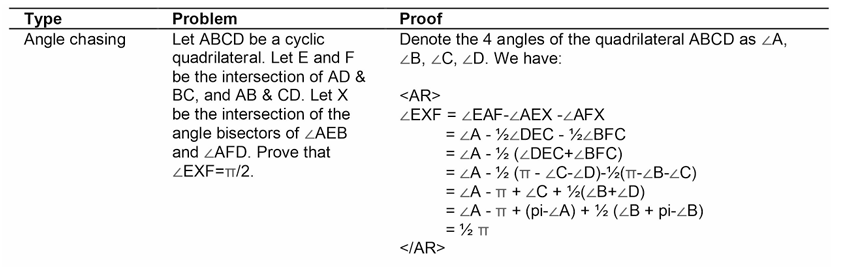
\includegraphics[width=0.6\linewidth]{figures/Examples of AR.png}
        \end{figure}
	
\end{frame}

\begin{frame}
        \frametitle{Synthetic-data-generation in AG}
        \begin{itemize}
            \item Synthetic Problems and Proofs:

            A synthetic problem and its solution are formed by the minimal premise and the corresponding subgraph.
        \end{itemize}

        \begin{figure}
            \centering
            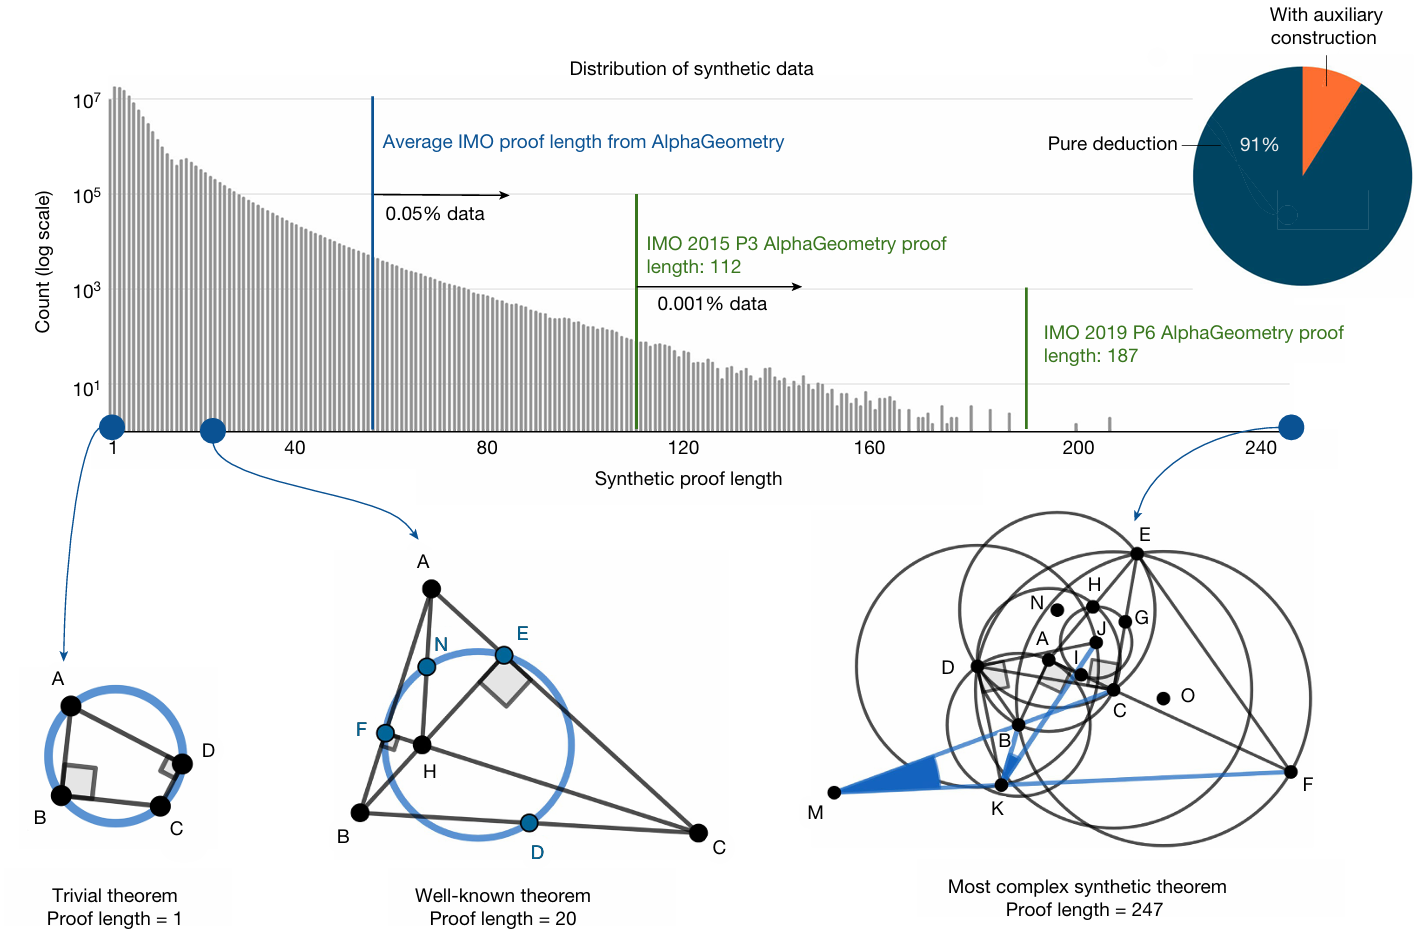
\includegraphics[width=0.6\linewidth]{figures/Constrcution of Data.png}
        \end{figure}

\end{frame}

\begin{frame}
        \frametitle{An Example of Problem solving in AG}
        \begin{figure}
            \centering
            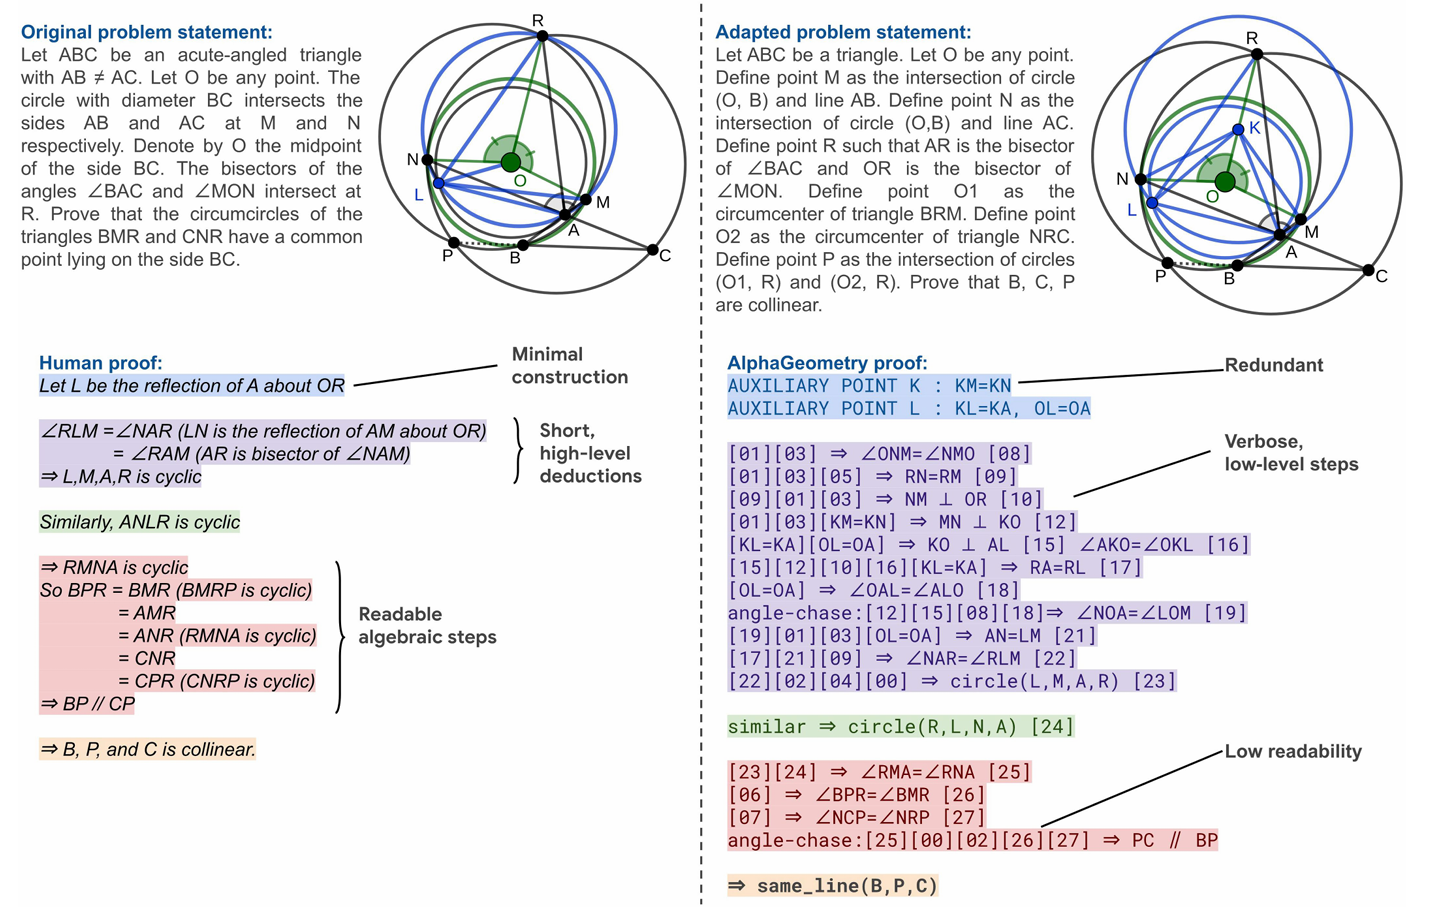
\includegraphics[width=0.8\linewidth]{figures/Example_AG.png}
        \end{figure}
	
\end{frame}

\begin{frame}
        \frametitle{A Following Work: AG2}
        \begin{itemize}
            \item A significantly improved version of AG1, achieving a gold-medalist level of performance on International Mathematical Olympiad (IMO) geometry problems, solving 84\% of the problems over the last 25 years, compared to the 54\% success rate of its predecessor.

            \item The main improvements of AG2 include:
            \begin{itemize}
                \item Expanded domain language: Added support for movements of objects, increasing the DSL coverage on IMO 2000-2024 geometry problems from 66\% to 88\%.
                \item Stronger and faster symbolic engine: Introduced an optimized rule set, better handling of double points, and a two-order of magnitude faster implementation in C++.
                \item Enhanced language model: Leveraged the Gemini architecture, trained on an order of magnitude larger and more diverse dataset.
                \item Advanced novel search algorithm: Introduced Shared Knowledge Ensemble of Search Trees (SKEST) that employs a knowledge-sharing mechanism to expand and accelerate the search process.
            \end{itemize}
        \end{itemize}

\end{frame}

\begin{frame}
        \frametitle{Evaluation on Benchmark}
        \begin{columns}
            \column{0.3\textwidth}
            \begin{itemize}
                \item AG1 and AG2, by integrating neural language models and symbolic reasoning engines, have made significant progress in solving Olympiad-level geometry problems, especially AG2
            \end{itemize}
            
            \column{0.7\textwidth}
            \begin{figure}
                \centering
                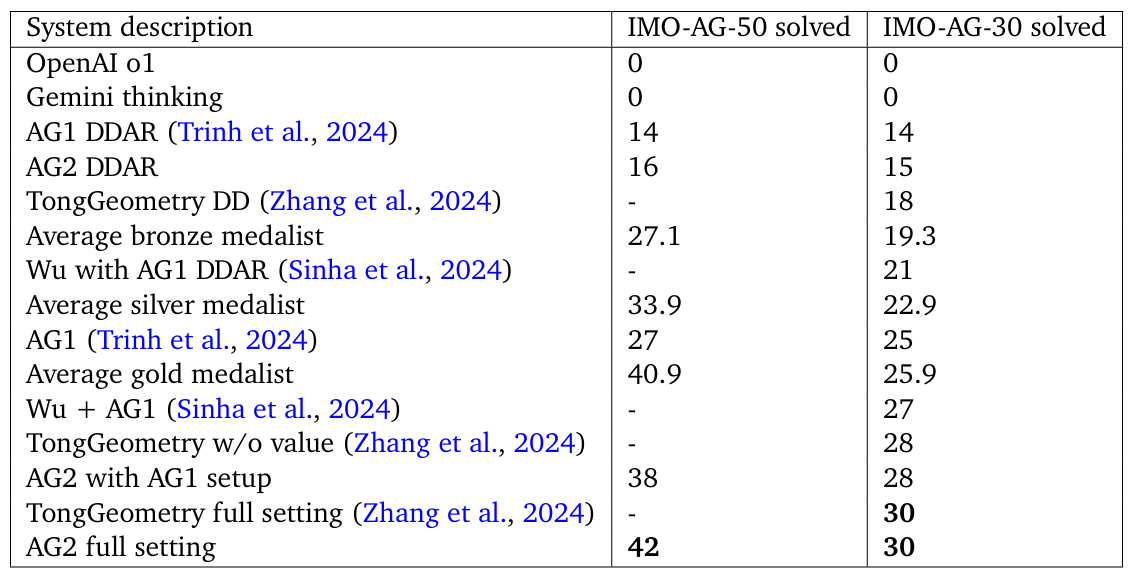
\includegraphics[width=0.9\linewidth]{figures/Evaluation.png}
            \end{figure}
        \end{columns}
        

\end{frame}

\section{Ongoing Work and Future Plans}

\begin{frame}
    \frametitle{Ongoing Work and Future Plans}
        \begin{itemize}
            \item \textbf{Ongoing Work}
            \begin{itemize}
                \item Reproduction the Result of AG: Since the code for AG is semi-open source and only includes the inference part, we are now reproducing the results of AG based on Newclid. % \footnote{Vladmir Sicca, Tianxiang~Xia et al., "Newclid: A User-Friendly Replacement for AlphaGeometry",2024}
                \item As of now, the speed of data generation has been increased by a factor of 3 to 10 times the original rate.
            \end{itemize}

            \item \textbf{Future Plans}
            \begin{itemize}
                \item Introduce new predicates and constructions to support more complex geometric problems;
                \item Optimize the algorithms of DD and AR;
                \item Generate auxiliary points based on previous proof steps rather than from the problem statement;
                \item Combine AG with Wu's method to gain a better performance;
                \item Utilize multimodal information to improve problem formalization and the generation of auxiliary constructions
            \end{itemize}
        \end{itemize}
\end{frame}

\section{References}
\begin{frame}
    \frametitle{References}
	\begin{thebibliography}{99}
        \bibitem{yang2023} Kaiyu~Yang, Aidan~M.~Swope, Alex~Gu, Rahul~Chalamala, Peiyang~Song, Shixing~Yu, Saad~Godil, Ryan~Prenger, and Anima~Anandkumar, {\sl LeanDojo: Theorem Proving with Retrieval-Augmented Language Models}, Oct.~27, 2023  
		
        \bibitem{trinh1} Trieu~H.~Trinh, Yuhuai~Wu, Quoc~V.~Le et al., {\sl Solving olympiad geometry without human demonstrations}, Jan.~18, 2024
		
        \bibitem{chervonyi2025} Yuri~Chervonyi, Trieu~H.~Trinh, Miroslav~Olšák, Xiaomeng~Yang, Hoang~Nguyen, Marcelo~Menegali, Junehyuk~Jung, Vikas~Verma, Quoc~V.~Le, and Thang~Luong, {\sl Gold-medalist Performance in Solving Olympiad Geometry with AlphaGeometry2}, Feb.~28, 2025
        
        \bibitem{sicca2024} Vladmir~Sicca, Tianxiang~Xia, Mathïs~Fédérico, Philip~John~Gorinski, Simon~Frieder, and Shangling~Jui, {\sl Newclid: A User-Friendly Replacement for AlphaGeometry}, Nov.~20, 2024

	\end{thebibliography}
\end{frame}

\end{document}